\documentclass{article} % For LaTeX2e
\usepackage{nips14submit_e,times}
\usepackage{hyperref}
\usepackage{url}
\usepackage{amsmath, amssymb, graphicx, algpseudocode, algorithm, amsthm}
%\documentstyle[nips14submit_09,times,art10]{article} % For LaTeX 2.09


\title{Representation Discovery for Kernel-Based
Reinforcement Learning}


\author{
Dawit H.~Zewdie \\
Learning and Intelligent Systems Group\\
MIT, CSAIL\\
Cambridge, MA 02139 \\
\texttt{dawit@alum.mit.edu} \\
%}
\And
%\author{
George Konidaris\\
Intelligent Robot Lab\\
Duke University\\
Durham, NC 27708\\
\texttt{gdk@cs.duke.edu} \\
}

\newenvironment{claim}[1][Claim]{\begin{trivlist}
\item[\hskip \labelsep {\bfseries #1}]}{\end{trivlist}}
\newenvironment{lemma}[1][Lemma]{\begin{trivlist}
\item[\hskip \labelsep {\bfseries #1}]}{\end{trivlist}}

% The \author macro works with any number of authors. There are two commands
% used to separate the names and addresses of multiple authors: \And and \AND.
%
% Using \And between authors leaves it to \LaTeX{} to determine where to break
% the lines. Using \AND forces a linebreak at that point. So, if \LaTeX{}
% puts 3 of 4 authors names on the first line, and the last on the second
% line, try using \AND instead of \And before the third author name.

\newcommand{\fix}{\marginpar{FIX}}
\newcommand{\new}{\marginpar{NEW}}

\nipsfinalcopy % Uncomment for camera-ready version

\begin{document}


\maketitle

\begin{abstract}
Recent years have seen increased interest in non-parametric reinforcement
learning.
There are now practical kernel-based algorithms for approximating
value functions; however, kernel regression requires that the underlying
function being approximated be smooth on its domain.
Few problems of interest satisfy this requirement in their natural representation.
In this paper we define \textbf{value-consistent pseudometric (VCPM)}, the
distance function corresponding to a transformation of the domain into a space where
the target function is maximally smooth and thus well-approximated by kernel regression.
We then present \textbf{DKBRL}, an iterative batch RL algorithm interleaving steps of
Kernel-Based Reinforcement Learning and distance metric adjustment.
We evaluate its performance on Acrobot and PinBall,
continuous-space reinforcement learning domains with discontinuous value functions.
\end{abstract}

\section{Introduction}

Kernel-based reinforcement learning (KBRL) methods  have recently
begun to receive significant research
attention \cite{kbrl,kbrl2,kbsf,ikbsf,pkbrl}. These
algorithms have the virtue of being non-parametric: their computational complexity
scales with the amount of data, rather than with the size of the state space; consequently,
they are a promising means of avoiding the so-called \textit{curse of dimensionality}, where
the number of parameters in a parametric representation of a general value function
scales exponentially with the dimensionality of the state space. 

Key to these algorithms is the use of kernel regression to extrapolate values.
Kernel regression is a smooth-function approximation technique that performs
all computation in terms of distance in the state space.

Kernel regression has difficulty modelling discontinuous functions.
This difficulty can be alleviated by adding more data, but doing so is often undesirable.
We show that changing the distance metric used in the
regression can efficiently resolve the difficulties.
Existing metric learning algorithms are not, in general, capable of dealing with
discontinuities.
We introduce the notion of a \textit{value-consistent pseudometric} (VCP) and show
that it allows kernel-regression to model discontinuous functions.
We then present a novel iterative algorithm for approximating the VCP,
and evaluate its performance on Acrobot and PinBall,
two reinforcement learning domains with discontinuous value functions.

\section{Background}

Reinforcement learning \cite{rlai} problems are typically formalized as 
Markov Decision Processes (MDPs) \cite{put},which can be described
by a tuple $\langle S,A,T,R,\gamma\rangle$, where
$S$ is a possibly infinite set of states, $A$ is a finite set of actions,
$T:S\times A\times S\to[0,1]$ is an expression of the probability
that a given action will result in a particular state transition
$R:S\times A\times S\to\mathbb{R}$ is an expression of the reward received
for each possible state transition, and
$\gamma$ is a discount factor specifying how much the agent prefers immediate
rewards to future ones.
The agent starts the process in some
start state, $s_0$, and chooses an action $a_t$ based on $s_t$ at every
time step $t$, causing the state to change to state $s_{t+1}$ with
probability $T(s_t,a_t,s_{t+1})$, and the agent to receive reward 
 $r_t = R(s_t,a_t,s_{t+1})$. 
The reward and transition functions are assumed to
be unknown; the agent must learn how to act by observing sample
rewards and transitions.
In this paper, we assume that the agent is given a batch of sample
transitions from which to learn.

The agent picks actions by a policy $\pi:S\to A$.
The total reward the agent can expect 
when following $\pi$ starting from state $s$ is denoted
$V^\pi(s) = E\left[\sum_i\gamma^i r_i|s_0 = s, a_i=\pi(s_i)\right]$.
The agent's objective is to maximize this \textit{return}, by finding
a policy, $\pi^*$, such that
$V^{\pi^*}(s) = \max_\pi V^\pi(s)$ for all states $s$.
It is convenient to think in terms of
the value of a state-action pair, $Q^{\pi}(s,a)$,
the expected return when taking action, $a$, in state, $s$,
then following $\pi$ forever after. $V^\pi(s) = \max_a Q^\pi(s,a)$

When the set of states is small and finite, an MDP can be efficiently solved
by value iteration, which uses dynamic programming to find $V$ and $Q$ satisfying
$$Q(s,a) = \sum_{s' \in S} T(s,a,s')\left[R(s,a,s') + \gamma V(s')\right].$$

Solving MDPs with continuous state spaces is less straightforward.
Popular techniques include LSTD \cite{lstd}, and Sarsa \cite{sarsa}
%, and fitted Q-iteration \cite{fqi}, all of
which try to approximate the value function parametrically.
With the right parametric form, these algorithms can produce high quality solutions
from very little data; however, no amount of data can help them produce a good
solutions when they assume the wrong form.

By contrast, non-parametric methods represent the value
function directly in terms of the data.
This avoids the need for assumptions about value function form
and allows the complexity of the fit generated to scale naturally with
the amount of data.
We are interested in improving KBRL, one particular non-parametric algorithm.
%Fitted Q-iteration \cite{fqi} cite[ernst] is a non-parametric method that exists
%but we do not discuss it further.

\subsection{Kernel-Based Reinforcement Learning}

KBRL \cite{kbrl} is a non-parametric value function approximation algorithm for
continuous MDPs.
It is a three-step process that solves the MDP using a set of sample
transitions.
The first step constructs a finite approximation of the MDP from the samples,
the second step solves that finite approximation, and the third step
interpolates that solution to the original state space.

KBRL takes as input a set of sample transitions, 
$S^a = \{ w^a_i = (s^a_i, r^a_i, \hat s^a_i)\ |\ i = 1, \ldots, n_a \}$, resulting from
each action, $a$. 
From these transitions, KBRL constructs a finite MDP,
$M'=\langle S',A,T',R',\gamma\rangle)$. 
The new state space, $S'$, is the set of sample transitions, so $|S'| = n = \sum_a n_a$. 
The new reward function is $R'(w^a_i, a', w^{a'}_j) = r^{a'}_j$.
The new transition function $T'$ is defined as 
\[
 T'(w^a_i, a', w^{a''}_j) = \left\{
  \begin{array}{lr}
    0 & \mathrm{if}\ a' \neq a'' \\
    \kappa_{a'}(\hat s^a_i, s^{a''}_j) &  \mathrm{otherwise,}
  \end{array}
\right.
\]
where $\kappa_a(\cdot, \cdot)$ is some similarity function constrained
to be nonnegative, decreasing in the distance between its two arguments,
and satisfying $\sum_i \kappa_a(s,s^a_i) = 1$ for all $s \in S$.
It is convenient to think of $\kappa$ as being the normalized
version of some underlying \textit{mother kernel}, $k$, so that
$\kappa_a(s,s^a_i) = \frac{k(b^{-1}d(s,s^a_i))}{\sum_j k(b^{-1}d(s,s^a_j))}$
where $d$ is a metric and $b$ is a bandwidth.
There is a bias-variance trade-off to be made when choosing $b$;
bias decreases with $b$ while variance increases \cite{kbrl}.
Except where stated otherwise, we use a Gaussian as our mother kernel throughout this paper.

There is work \cite{kbrl2} exploring the possibilities for similarity
functions (trees, nearest neighbours, and grid-based approximations),
but all of it uses Euclidean distance, $d_{\mathrm{Euc}}$, as the metric.
The justification is that the value function is assumed smooth---that nearby
points have similar values.
When it uses $d_{\mathrm{Euc}}$, KBRL can be seen as using local averaging
to approximate the transition, reward, and Q-value functions.
In the next section we show what happens when the smoothness assumption is
not met.

KBRL solves for $V'$, the value function of $M'$ using some finite MDP solver
then generalizes it to $M$ using the equation
$$Q(s,a) = \sum_{w^a_i \in S^a}
\kappa_a(s,s_i^a)\left[r_i^a + \gamma V'(w^a_i)\right].$$

Note that the size of the finite model, $M'$ constructed by KBRL is equal to the
number of sample transitions.
This makes solving it computationally intensive, even when using a sparse
kernel; however,
an approximate solution to $M'$ can be found
efficiently if its transition probability matrix is replaced by a low-rank
approximation \cite{pkbrl}. Kernel-based stochastic factorization (KBSF)
takes advantage of this property, using a stochastic factorization of the
matrix as the low-rank approximation.
KBSF takes time linear in the amount of data and a constant amount
of space that depends only on the desired approximation coarseness.
Though we only provide proofs and results for KBRL, the ideas presented
in this paper can also be applied to KBSF.

\section{Importance of the Right Metric}
Because of its smoothness assumptions, KBRL is not well suited
for solving MDPs whose value functions have cliffs.
To see why, consider \textit{TWO-ROOM},
a simple MDP presented in Figure \ref{tworoom}.
It describes a world with two rooms connected by doorway.
The agent can freely move through the open space of the world but cannot
go through the wall.\footnote{For the purposes of discussion, assume the agent can move in any
direction or choose to stay in place (making for an infinite set of actions).}
 A region in one room is marked as the goal.
The agent receives a reward of $0$ when inside the goal and $-1$ otherwise.

\begin{figure}[!!!ht]
  \centering
    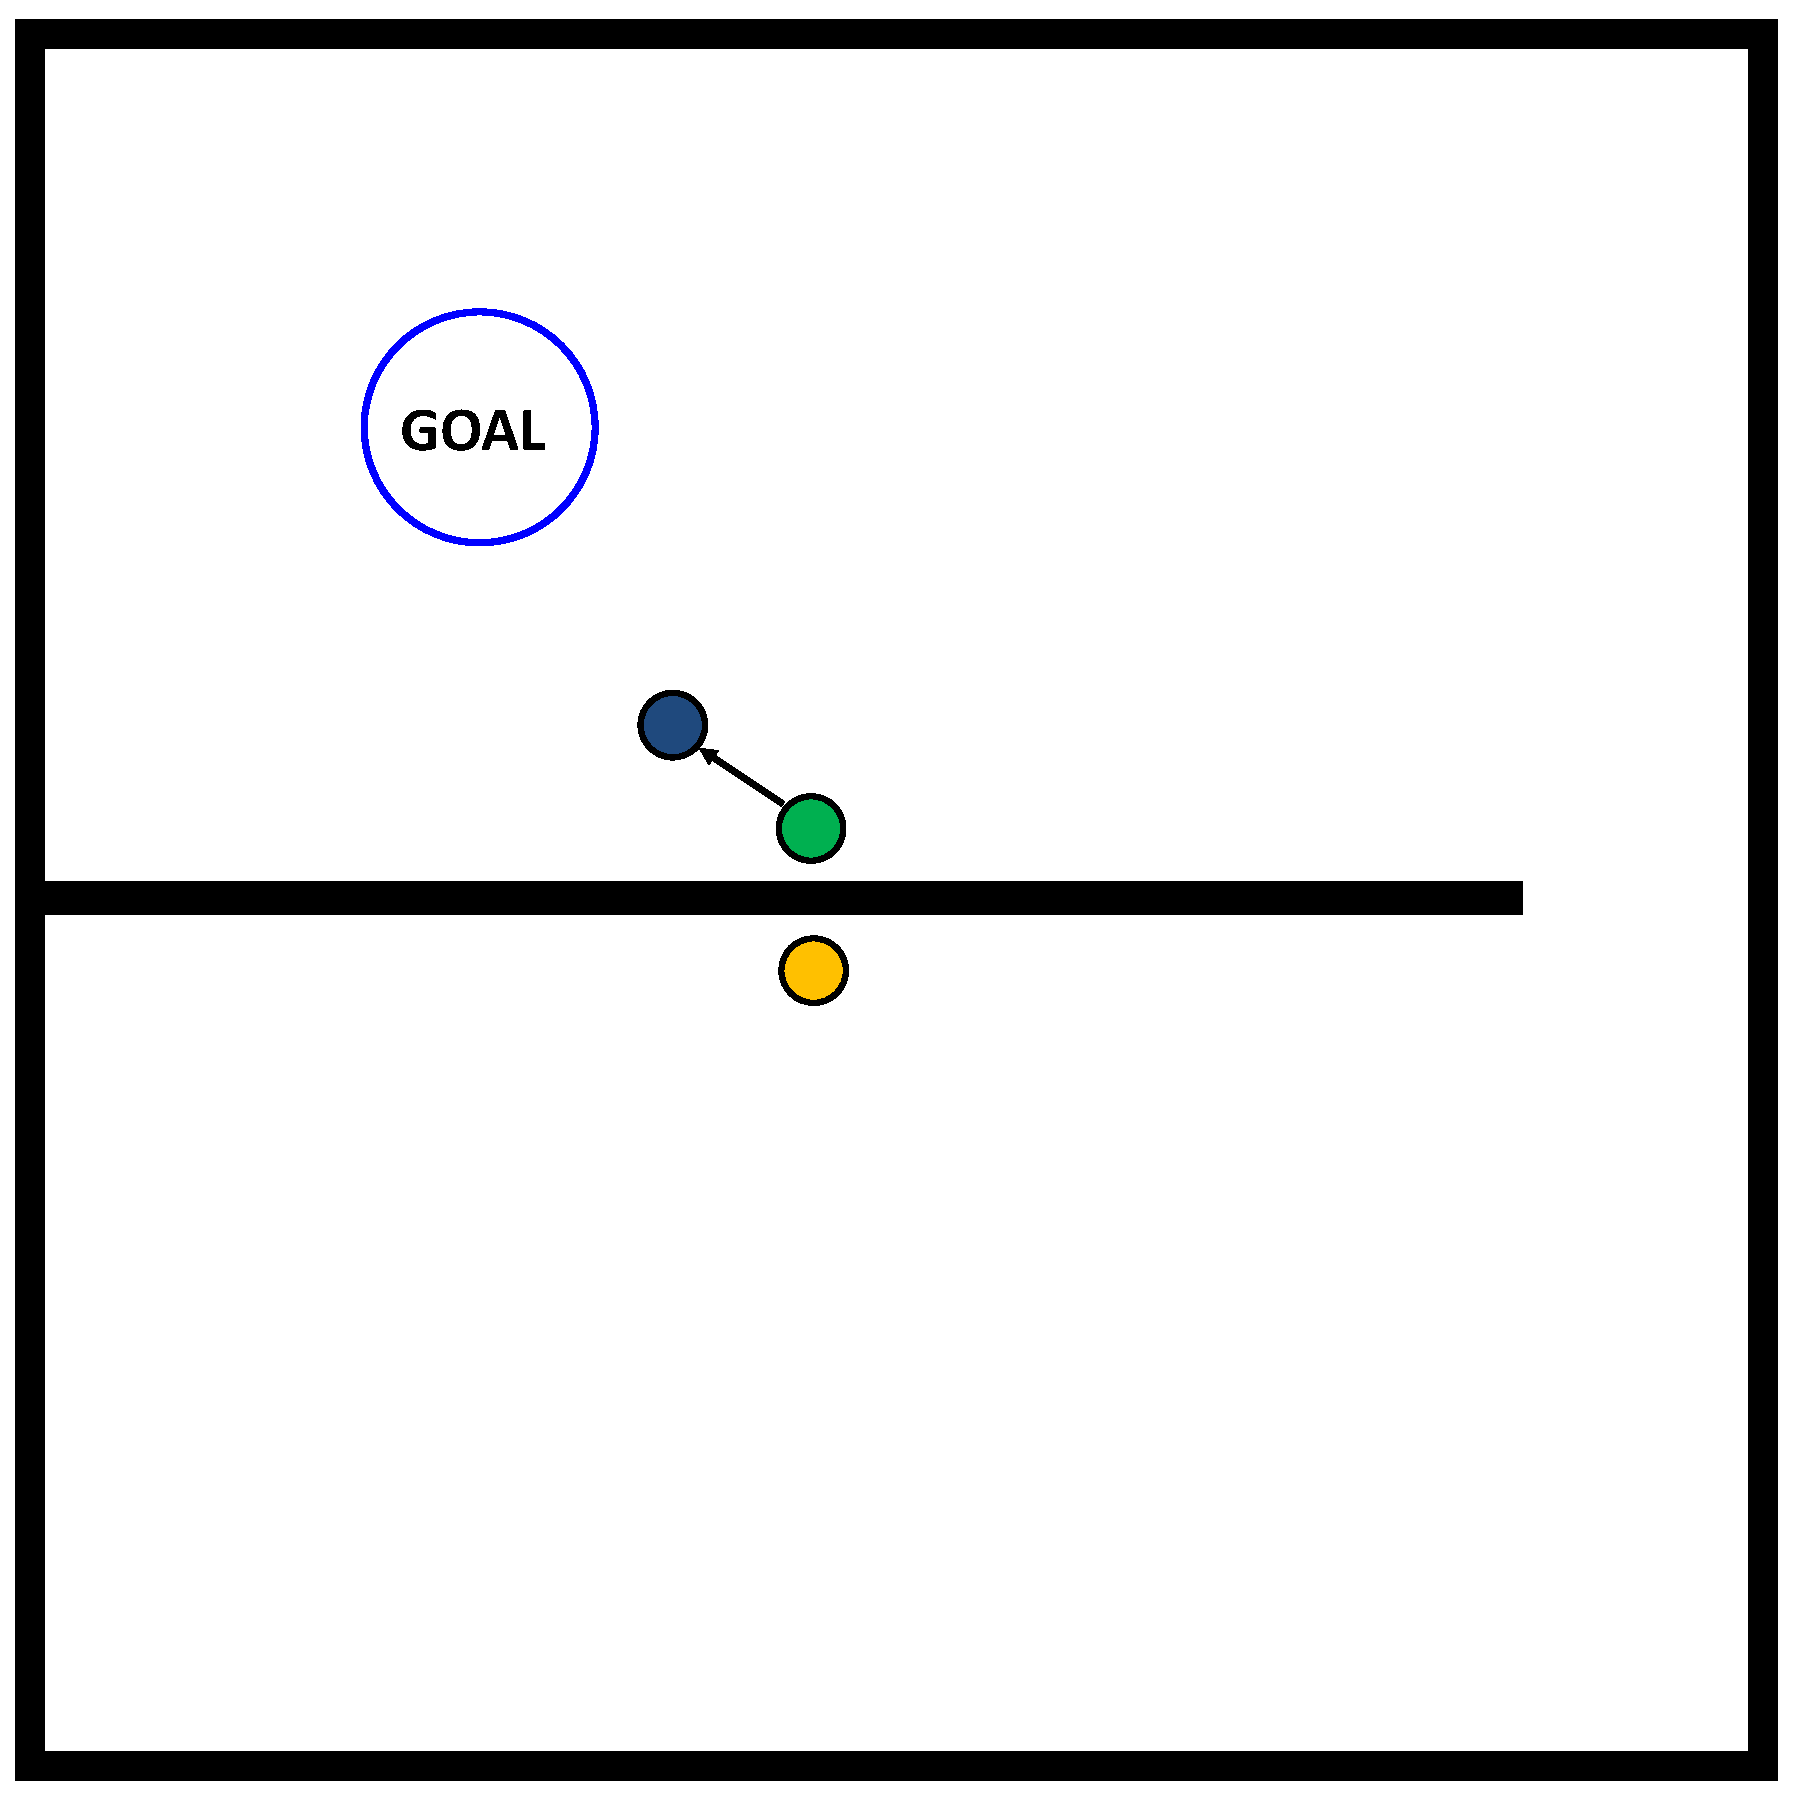
\includegraphics[width=60mm]{../writeup/figs/tworoom.pdf}
  \caption[State Space]
{The state space of \textit{TWO-ROOM}. There is a sample transition in the top room
and state near the sample in the bottom room}
  \label{tworoom}
\end{figure}

The  optimal policy in \textit{TWO-ROOM} is to navigate directly to the goal.
Thus, the value of a state, $s$, is decreasing in the length of the shortest path
from it to the goal, $d_{\mathrm{TR}}(s,g)$ (where $d_{\mathrm{TR}}$ denotes
shortest-path metric).
States that are physically close together but on opposite sides of the
wall have starkly different values. To solve \textit{TWO-ROOM},
one must faithfully represent this steep drop in value across the wall. 

For KBRL to represent the value cliff, it must be run with a small bandwidth.
Compensating for the resulting variance requires a large set of sample transitions,
making the domain challenging for KBRL.
However, if we use $d_{\mathrm{TR}}$ instead of $d_{\mathrm{Euc}}$ as the
metric in the mother kernel, \textit{TWO-ROOM} becomes easily solvable with a large bandwidth
and small data set.
Since the value function is smooth with respect to $d_{\mathrm{TR}}$ we can
use large bandwidths with no risk of averaging across the wall.

\begin{figure}[!htb]
  \minipage{0.30\textwidth}
    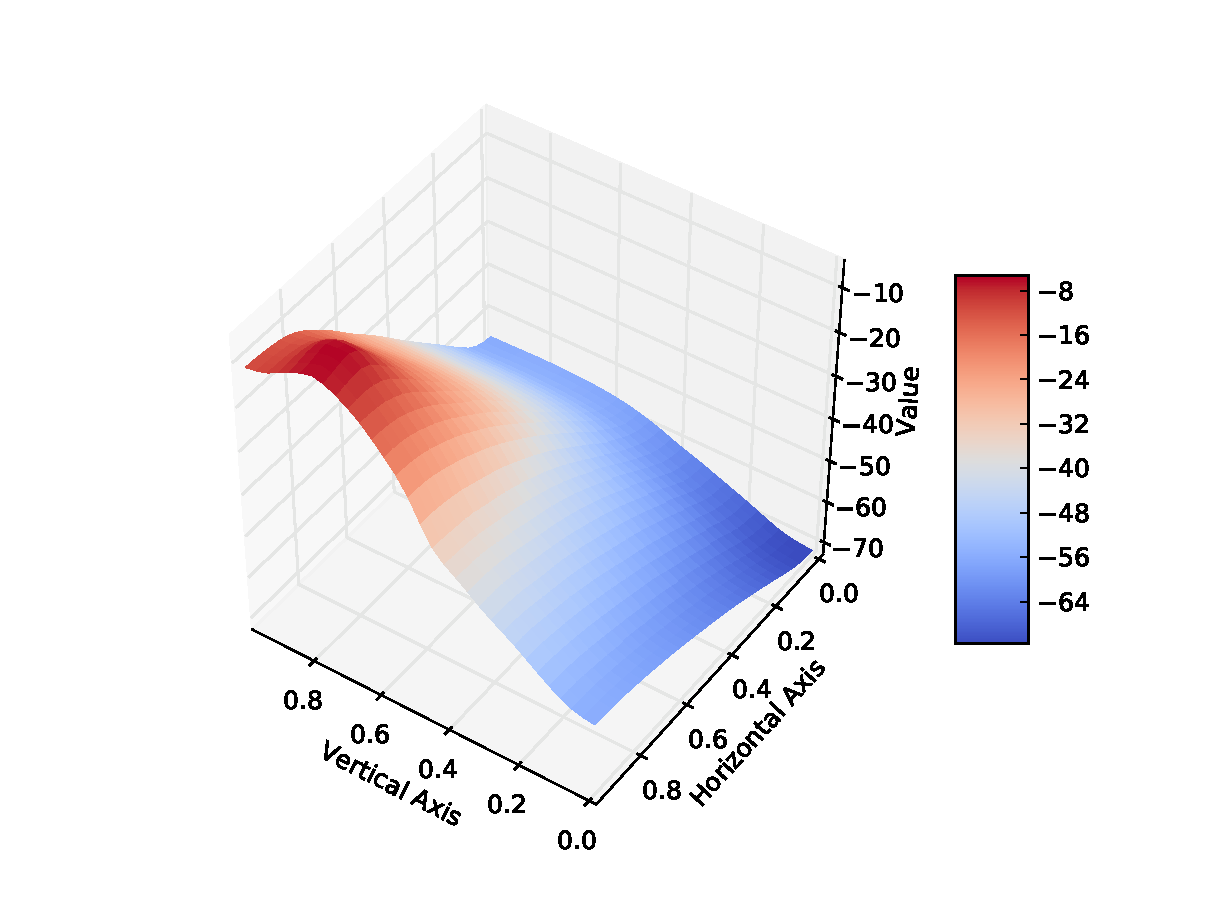
\includegraphics[width=\linewidth]{../writeup/figs/blur2rmvf.pdf}
  \endminipage\hfill
  \minipage{0.30\textwidth}
    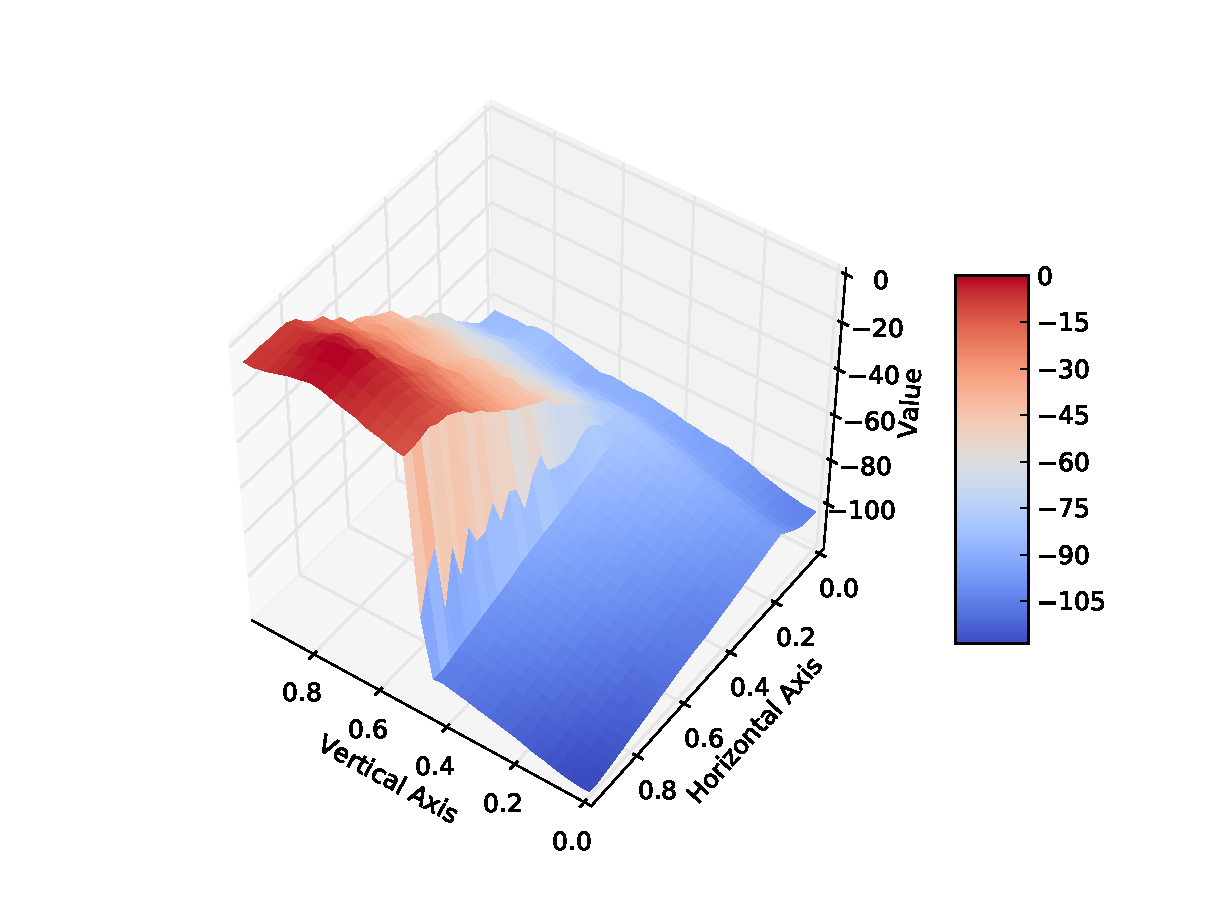
\includegraphics[width=\linewidth]{../writeup/figs/true2rmvf.pdf}
  \endminipage\hfill
  \minipage{0.30\textwidth}
    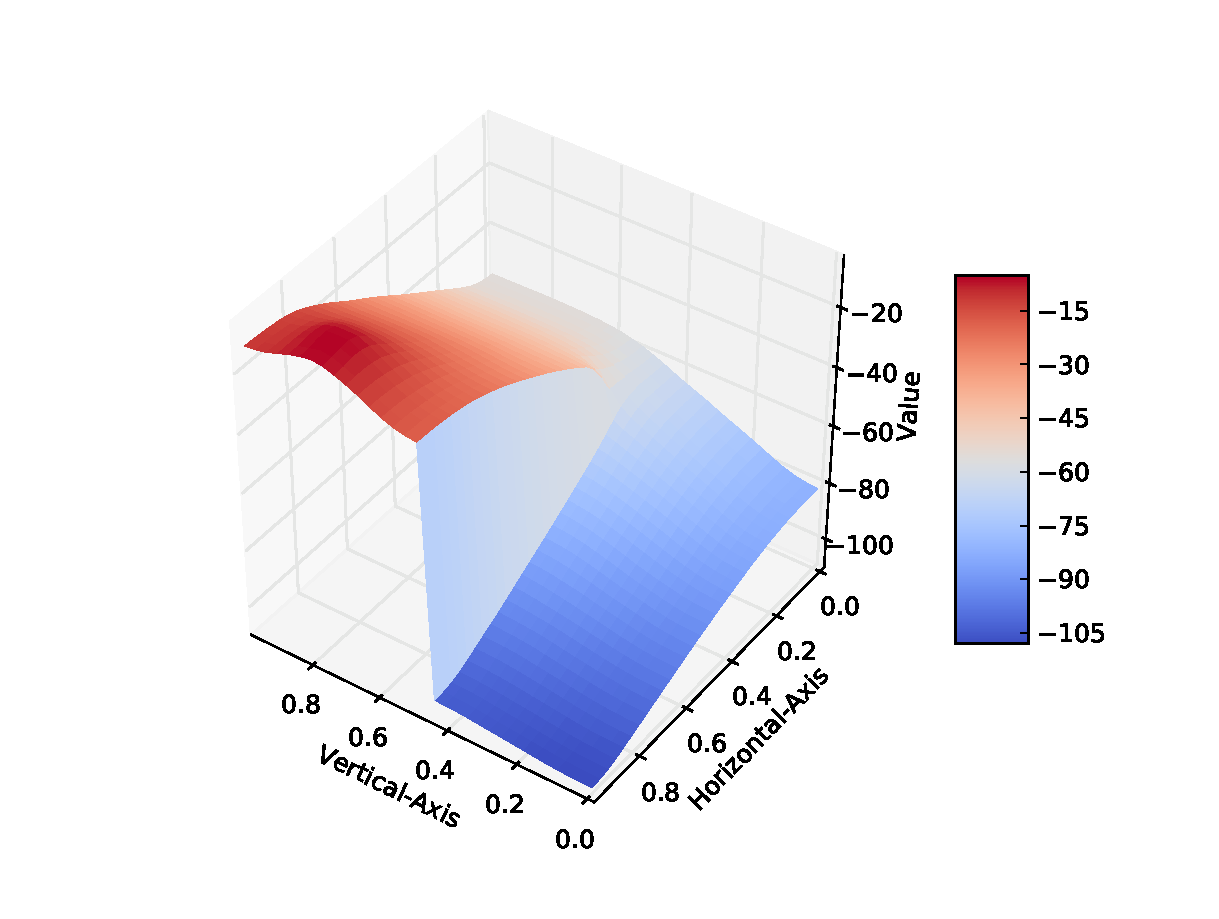
\includegraphics[width=\linewidth]{./figs/trdfvf.pdf}
  \endminipage\hfill
\caption[Importance of Representation]
{Left to right: \textit{TWO-ROOM}'s
 value function estimated with $d_{Euc}$ and $b=.06$; with $d_{Euc}$ and
$b=.01$; and with $d_{TR}$ and $b=.06$}
\label{trgraphs}
\end{figure}

We tried solving \textit{TWO-ROOM} with different combinations of bandwidth and metric,
holding the training set fixed \ref{trgraphs}.
When running KBRL with a large bandwidth and the Euclidean metric,
the value cliff is completely smoothed out.
The resulting policy has the agent attempt to walk through the wall.
With a small bandwidth, KBRL finds the correct overall shape for
the value function, but there are some ripples that appear as artefacts of
the small bandwidth.
The resulting policy has the agent reach the goal on a path that zigzags 
around the shortest path.
Running KBRL with $d_{\mathrm{TR}}$ and a large bandwidth produces the
correct shape for the value function without any ripples.
The resulting policy takes the agent to the goal along the shortest path.

The manifold of the \textit{TWO-ROOM} state space is a square with
a line segment cut out of it.
The value function is smooth on the manifold but discontinuous in Euclidean space.
Thus, using distance on the manifold instead of Euclidean distance makes kernel
regression work better.
Domains like \textit{TWO-ROOM} have been used to motivate representation discovery in
parametric reinforcement learning, most notably by
Proto-Value Functions \cite{pvf} which use the eigenfunctions of the manifold as a basis.

The discontinuity in \textit{TWO-ROOM}'s value function comes from the local
connectivity of the state space, but local connectivity is not the only factor that affects
value function smoothness.
Consider, for instance, a modification to \textit{TWO-ROOM} where the wall is replaced
by a region of low reward.
The agent can freely move through this region, but would get a better return
by going around it.
This modification removes the connectivity issues (the state space manifold is
Euclidean space) but the value function still has the same discontinuity.
Now consider a modification where the agent can jump over the wall if it has
enough momentum. With this modification, two states that are close to each other
\footnote{Note that here we are measuring distance in phase space. Two states are nearby if
they have similar position and velocity.}
and far from the wall can have very different values depending on whether the agent
is on a trajectory that can hurdle the wall.
This modified version of \textit{TWO-ROOM} has a value function discontinuity that extends
beyond the wall and no local information can help distinguish the states it separates.
Neither $d_{Euc}$ nor $d_{\mathrm{TR}}$ do particularly well here.

The cases above show that a good metric must consider more than just local
state space topology;
it must also account for global dynamics and the reward structure of the MDP.
In some sense, knowing the right metric requires already knowing the value function.
The next section identifies the ideal metric and provides an algorithm for approximating it.

\section{Value-Consistent Pseudometrics}
KBRL uses kernel regression to approximate the Q-values of an MDP.
It does this using kernels of the form
$\kappa_a(s,s')=c_a\cdot k(\frac{d_{\mathrm{Euc}}(s,s')}{b})$, where $c_a$ is a
normalizing constant.
We are interested in finding a new metric $d'$ to replace $d_{\mathrm{Euc}}$ in
the regression.
To keep things simple, we begin by removing the reinforcement learning component
of the problem and only considering regression.

\subsection{Transforming to Improve Regression}
The problem statement of regression is as follows: given a set of training
points, $D = \{(x_i,y_i)\ |\ i = 1, \ldots, n\}$, of point-value pairs with
$y_i = f(x_i)$ for some $f : X \to \mathbb{R}$,
produce a function $\tilde f$ that approximates $f$ well, for some measure of
approximation quality.\footnote{We assume that $X$ is a compact, connected subset
of $\mathbb{R}^m$; 
%that $f$ is piecewise Lipschitz-continuous;
and that $\max_i y_i = y_{max} \neq y_{min} = \min_i y_i$.
From these assumptions it follows that $f$ has
distinct extrema on $X$; we refer to these as $f_{max}$ and $f_{min}$.
We refer to the diameter of $X$ under metric $d$ as $\Delta_X(d)$}

Regression with a kernel estimator \cite{kern} produces the estimate
$\tilde f(x) =
\frac{\sum_i k(b^{-1}d_{\mathrm{Euc}}(x-x_i))y_i}{\sum_i k(b^{-1}d_{\mathrm{Euc}}(x-x_i))}$.
In Section 3, we found that replacing $d_{\mathrm{Euc}}$
with a function that varies more closely with $f$ can produce better results.
The function that varies most closely with $f$ is the pseudometric\footnote{$d^*_f$
is a pseudometric because it doesn't satisfy $d^*(x,x') \implies x=x'$; in the
supplementary matrials we show that it is safe to use $d^*_f$ as a metric in kernel
regression.} $d^*_f(x,x') = |f(x)-f(x')|$.
The diameter of $X$ under $d^*_f$ depends on $f$.
We can remove this dependence using the scalar
$\mu_f = \frac{\Delta_X(d_{\mathrm{Euc}})}{f_{max}-f_{min}}$ to make $d_f(x,x') = \mu_f d^*_f(x,x')$,
a pseudometric with the same diameter as $d_{\mathrm{Euc}}$.
$d_f$ is the most natural choice for replacing $d_{\mathrm{Euc}}$ in the regression.
We call $d_f$ the \textbf{value-consistent pseudometric (VCPM)} for $f$ on $X$.

Unfortunately, to use $d_f$ in the regression one would need to already know $f$.
Our workaround is an iterative algorithm that interleaves steps of regression
and metric learning to approximate the VCPM for $f$ on $X$.
We start with an initial metric $d_0 = d_{\mathrm{Euc}}$ and use the kernel estimator to
produce an estimate $f_1$.
We then use $f_1$ and $d_0$ to produce a new metric $d_1$ that corresponds
to a representation of $X$ where $f_1$ is smoother.
We then use $d_1$ in our kernel estimator to get a new estimate $f_2$ and repeat until
the approximation stops improving.

The metric $d_i$ should be a relaxation of $d_{i-1}$ towards $d_{f_i}$,
the VCPM for $f_i$ on $X$.
One way to do this would be to choose
$d_i(x,x') = c_0\sqrt{d_{i-1}(x,x')^2 + \alpha^2d_{f_i}(x,x')^2}$,
where $c_0$ is a diameter preserving constant and $\alpha > 0$ is a relaxation rate.
Note that even though $d_{f_i}$ is a pseudometric, each $d_i$ is guaranteed to
be a valid metric on $X$ because of the dependence on $d_{i-1}$.

The effect of varying $\alpha$ is discussed in the Appendix.
The diameter preserving $c_0$ satisfies $\frac{1}{\sqrt{1+\alpha^2}} \leq c_0 \leq 1$ and is difficult
to calculate exactly, so we assume the lower bound.
Calculating $d_{f_i}$ requires knowing the extrema of $f_i$, which are also difficult to compute
but known to be bounded by $y_{max}$ and $y_{min}$;
we use these bounds in place of the exact values.
With these two heuristics, the metric will underestimate some distances.
Underestimating distances is equivalent to using a larger bandwidth,
which is an acceptable trade-off for the performance improvement.

With these adjustments, our relaxation of the metric becomes
$$d_i(x,x') = \frac{1}{\sqrt{1+a^2}}\sqrt{d_{i-1}(x,x')^2 + \left(\alpha \Delta(d_{\mathrm{Euc}})
\frac{f_i(x) - f_i(x')}{y_{max}-y_{min}}\right)^2}.$$

This relaxation can be viewed as a transform on $X$
compressing it where $f_i$ is flat and stretching it where $f_i$ is steep.
This transform warps the $m$-dimensional $X$ through $m+i$ dimensions
in such a way that $f_i$ becomes smoother.
For this reason, we call it a \textbf{Dimension-Adding 
Wrinkle-Ironing Transform (DAWIT)} \cite{thesis}.
Appendix A discusses the geometric interpretation of the transform in more detail.

For reasons explained in Appendix A, we refer to  ``kernel regression
augmented to learn a metric by DAWIT'' as FDK.
We are able to demonstrate a number of properties of FDK.
We have experimental evidence\footnote{see Appendix B} that the best fit does not always occur
in the limit.
We also have proof that: in the limit of infinite data and a bandwidth that shrinks at an appropriate rate,
the metric learned converges to the VCPM of $f$ on $X$;
for a fixed bandwidth and dataset, iterating until convergence produces a piecewise flat
approximation of $f$;
the number of pieces in the piecewise flat approximation varies inversely with $b$.

\begin{claim}
In the limit of infinite data and a bandwidth that shrinks at an
admissible rate\footnote{An admissible shrinkage rate \cite{kbrl}
is one where the bandwidth goes to zero but slowly enough (relative to the data increase)
to avoid creating an undesirable rise in variance.},
performing FDK to convergence with any $\alpha > 0$ will produce the VCPM of the function being approximated.
\end{claim}
\begin{proof} (sketch) We show this in two parts: First we show that repeatedly applying
DAWIT with the same function produces a sequence of metrics converging to the
VCPM for that function on its domain. Next, we use the
convergence properties of kernel regression to show that FDK also possesses the property.

Part 1: The metric produced by DAWIT on iteration $j$ satisfies
$$d_j(x_1, x_2) = 
\sqrt{\frac{d_{j-1}(x_1, x_2)^2 + \alpha^2\mu_{f}^2
\cdot(f(x_1) - f(x_2))^2}{1 + \alpha^2}}$$
$$= \sqrt{\frac{d_0(x_1, x_2)^2}{(1+\alpha^2)^j} + \alpha^2\mu_{f}^2
\cdot(f(x_1) - f(x_2))^2\sum_{i=1}^j\frac{1}{(1 + \alpha^2)^i}}.$$

As $j \to \infty$, the term involving $d_0$ goes to zero
exponentially quickly and the summation on the right converges to
$\alpha^{-2}$.
It follows that
$$\lim_{j\to \infty} d_j(x_1, x_2) = \mu_{f}\cdot(f(x_1) - f(x_2))$$
which is the VCPM for $f$ on $X$.

Part 2: As the size of the dataset increases and the bandwidth decreases at an admissible rate,
the first estimate, $f_0$, produced by kernel regression converges to $f$. It follows that
the metric $d_1$ produced by DAWIT converges to a relaxation towards $d_f$ and subsequent
iterations of FDK resemble DAWIT repeated with the same function which, as we showed above,
converges to the VCPM for the function on its domain.
\end{proof}
The proof above shows that in the limit, FDK produces the pseudometric we identified as the ideal.
Next we show the convergence properties of FDK by characterizing the fixed points of FDK.
A pseudometric $d$ is a \textbf{fixed point} of FDK on dataset $D$ if performing a round of DAWIT
with $d_{i-1}=d$ (and $\tilde f_i$ being the result of kernel regression with $d_{i-1}$)
produces $d_i=d$.
\begin{lemma}A pseudometric $d$ is a fixed point of FDK if and only if the function $\tilde f$ created by
performing kernel regression using $d$ satisfies
$d(x_i, x_j) = \mu_{\tilde f}|\tilde f(x_i) - \tilde f(x_j)|$ for all $x_i, x_j \in D$.
\end{lemma}
The proof of this lemma is some straightforward arithmetic substituting into the equation for DAWIT;
it is omitted in the interest of space.
Next, we say a metric $d$ is an 
\textbf{attractive fixed point} of FDK
if there exists $\epsilon > 0$ such that starting FDK from any pseudometric $d_0$ satisfying
$|d_0(x,x') - d(x,x')| < \epsilon$ for all $x, x' \in X$, produces a sequence of converging to $d$.
The set of attractive fixed points is the set of pseudometrics to which FDK can converge.

\begin{claim}
For a metric, $d$ to be an attractive fixed point, the function $\tilde f$ resulting from doing
kernel regression with $d$ must be flat at $x_i$ for every $x_i \in D$.
\end{claim}
\begin{proof}(by contradiction)
Assume $d$ is an attractive fixed point of FDK for a given dataset $D$ such that $\tilde f$
is not flat at some $x_i \in D$. Assume WLOG that $i=1$.
$\tilde f$ being non-flat at $x_1$ means in any neighbourhood of $x_1$
there is some $x$ such that
$\tilde f(x) \neq \tilde f(x_1)$.
Note that this can only happen if $d(x,x_1) \neq 0$.

Given some $\epsilon$, Let $x^*$ be a point such that: $(x^*, f(x^*)) \notin D$;
$d(x^*,x_1) < \epsilon$; and $\tilde f(x^*) \neq \tilde f(x_1)$.
Let $d'$ be the pseudometric satisfying $d'(x,x^*) = d(x,x_1)$ for all $x$
and $d'(x,x') = d(x,x')$ for all $x, x' \neq x^*$.
The approximation $\tilde f'$ that results from using $d'$ in kernel regression
is identical to $\tilde f$ except at $x^*$, where
$\tilde f'(x^*) = \tilde f(x_1)$ (since $x^*$ is not in $D$ it has no influence over the regression).
It follows that $\tilde f'$ satisfies the constraints for $d'$ to be a fixed point.
Therefore $d$ does not attract $d'$ and cannot be an attractive fixed point.
\end{proof}

An implication of the claim above is that, in the limit, neighborhoods of points in the dataset get collapsed
into singularities. The supplementary materials provide intuition about how this happens.

In practice, we find that approximation error typically goes down then up,
and the metric that minimizes it is found after just a handful of iterations.
We also find that our augmented kernel regression is  very well suited for modelling
discontinuities like the one in \textit{TWO-ROOM}'s value function.
Appendix B provides empirical data about fit quality.

\begin{claim}When performed using a kernel, $k$, with compact support having
bandwidth,
$b < \frac{\Delta_X}{c}$, for some integer, $c$, FDK has an 
attractive fixed point with $c + 1$ singularities.\end{claim}

\begin{proof}(by construction)
Consider the dataset $D = \{(x_i,y_i)\ |\ i = 0\ldots c\}$ with $x_i=y_i=i$ produced
from a function $f: [0,c] \to \mathbb{R}$.
Let $d$ be the pseudometric such that $d(x_i, x_j) = d_{\mathrm{Euc}}(x_i, x_j)$
for all $i,j \in {0,\ldots, c}$ and $d(x,x_0) = 0$ for all $x \notin \{x_0, \ldots, x_c\}$.

First, we show that $d(x)$ is a fixed point.
Let $\tilde f$ be the function produced by kernel regression using $d$ as the metric.
Solving for $\tilde f$ gives $\tilde f(x)=\sum_j k(x,x_j)y_j$.
Because of the constraints on the bandwidth, $k(x_i,x_j)=0$ for all $i \neq k$, thus
$\tilde f(x_i) = y_i = x_i$ for all $i$ and $\tilde f(x) = y_0 =x_0$ for all $x \notin \{x_0, \ldots, x_c\}$.
$\tilde f$ is a line though all $c+1$ points in $D$.
By our lemma, this makes it a fixed point.

To show that $d_(x)$ is attractive, we consider a new pseudometric that is a perturbation of $d$.
Let $d_0$ be a pseudometric such that $|d(x,x') - d_0(x,x')| <
\frac{\Delta(X)}{c} - b$ for all pairs of points $(x,x')$ in $X$.
The $\tilde f_0$ that results from kernel regression using $d_0$ satisfies
$\tilde f_0(x) = \tilde f(x)$ because the perturbations were made
small enough that kernels centred on each $x_i$ still do not overlap.
During the metric learning step, DAWIT produces the metric
$d_1(x,x') \propto \sqrt{d_0(x,x')^2 + \alpha^2\mu^2(\tilde f(x) - \tilde f(x'))^2}
= \sqrt{d_0(x,x')^2 + (\alpha\mu d(x,x'))^2}$.
Note that $d_1$ is a relaxation towards $d$.
Since $d_1$ satisfies the constraints we placed on $d_0$, it follows that
$d_2, d_3, \ldots$, are also relaxations to $d$ and that the sequence ${\{d_i\}}$
converges to $d$, making $d$ an attractive fixed point.
\end{proof}

The proof above shows that the number of pieces in the piecewise flat approximation
generated in the limit of FDK is inversely proportional to the bandwidth used.
The proof can be extended to deal with kernels with infinite support.

\subsection{Transforming to Improve Reinforcement Learning}
Now that we have an extension of kernel regression capable of modelling
a wider class of functions, we are ready to apply it to reinforcement learning.

It is tempting to think that $d_{V^{\pi^*}}$, the VCPM for $V^{\pi^*}$, is the ideal pseudometric.
This is not the case; $d_{V^{\pi^*}}$ corresponds to an abstraction where all states with the same
value are mapped to the same abstract state.
Such an abstraction discards information about the optimal action.
What we need is an abstraction where only states with the same Q-values are mapped to the
same abstract state.

We can produce such an abstraction by using the VCPMs for the Q-values.\footnote{We
use $Q^a$ to refer to the function $Q^a(s) = Q^{\pi^*}(s,a)$.}
For each action $a$ we want
$\kappa_a(s,s^a_i) = \frac{k(b^{-1}d_{Q^a}(s,s^a_i))}{\sum_j k(b^{-1}d_{Q^a}(s,s^a_j))}$.
Note that we are using a different pseudometric in the kernel for each action.
Using the VCPMs for the Q-values corresponds to a $Q^*$-irrelevance abstraction;
it satisfies $\Phi(s) = \Phi(s') \implies Q^{\pi^*}(s,a) = Q^{\pi^*}(s',a)\ \forall a$
since $\|\Phi(s) - \Phi(s')\| = 0 \iff d_{Q^a}Q(s,s') = 0\ \forall a \iff
Q^{\pi^*}(s,a) = Q^{\pi^*}(s',a)\ \forall a$.
Acting optimally with respect to Q-values in a $Q^*$-irrelevance abstraction
results in optimal behaviour in the ground MDP \cite{lietal}.

Now that we have identified the desired abstraction, we can construct an algorithm to
approximate it.
As we did for regression, we start from the Euclidean metric and iteratively estimate
the Q-values (with KBRL) and update our metrics (with DAWIT).
Algorithm 1 describes the process.

\begin{algorithm}
\caption{DAWIT-KBRL}\label{dkbrl}
\begin{algorithmic}[1]
\Procedure{DKBRL}{$S',\ b$}
	\State $d^a_0 \gets d_{\mathrm{Euc}}\ \forall a$
	\State $i \gets 0$
	\Repeat
		\State $Q_{i} \gets \mathrm{KBRL}(S', b, d_{i})$
                \For{$a \in A$}
                    \State $d^a_{i+1} \gets \mathrm{DAWIT}(d^a_i, Q^a_{i})$
                \EndFor
		\State $i \gets i+1$
	\Until{Policy stops improving.}
	\State \textbf{return} $Q_{i-1}$
\EndProcedure
\end{algorithmic}
\end{algorithm}

In practice we found that it was rarely worth doing more than five
iterations of DKBRL.
There is one important detail that is worth mentioning;
%First, note that the algorithm presented above learns Q-values from
%scratch on every iteration;
%A useful optimization would be to use the Q-values from the previous
%iteration as a starting point for the value iteration.
%First is that, the stopping criterion is to perform policy evaluation.
the algorithm reuses the same dataset on each iteration because
the problem formulation is to learn from a batch of sample transitions.
Were we free to collect fresh data between iterations, we would want the sampled
points to be uniformly distributed with respect to the latest metric.
Doing so is necessary for KBRL's correctness guarantees.
Uniform coverage with the learned metric is equivalent to concentrating samples in the
regions of state space where the Q-values are steep, which is sensible
because that is where the Q-values tend to be poorly approximated.
In \textit{TWO-ROOM}, sampling uniformly from the transformed space corresponds
to choosing more samples along the wall.

We ran DKBRL on \textit{TWO-ROOM} with a large bandwidth ($b = .06$) to see if it
could identify the wall.
The results were successful; DKBRL was able to learn a metric that separated
states on opposite sides of the wall.
To visualize the metric, we sampled some points in the state space, calculated
all-pairs-shortest-paths, and performed multidimensional scaling \cite{mds} to get a 2D projection.
Figure \ref{eyec} shows the projection resulting from the metric for 
one action; the projections for the other actions were similar.

\begin{figure}[!htb]
  \minipage{0.32\textwidth}
    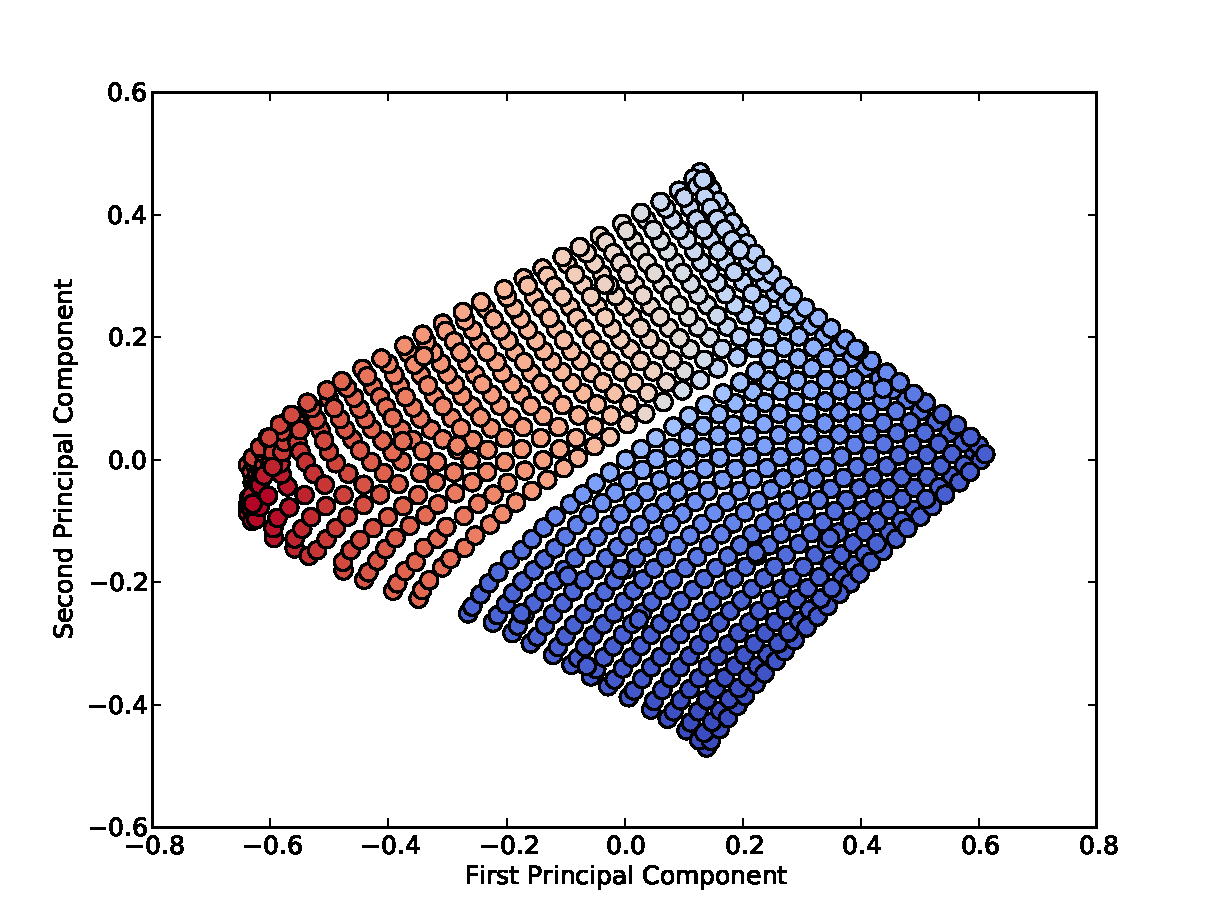
\includegraphics[width=\linewidth]{../writeup/figs/chap4/2rmop1.pdf}
  \endminipage\hfill
  \minipage{0.32\textwidth}
    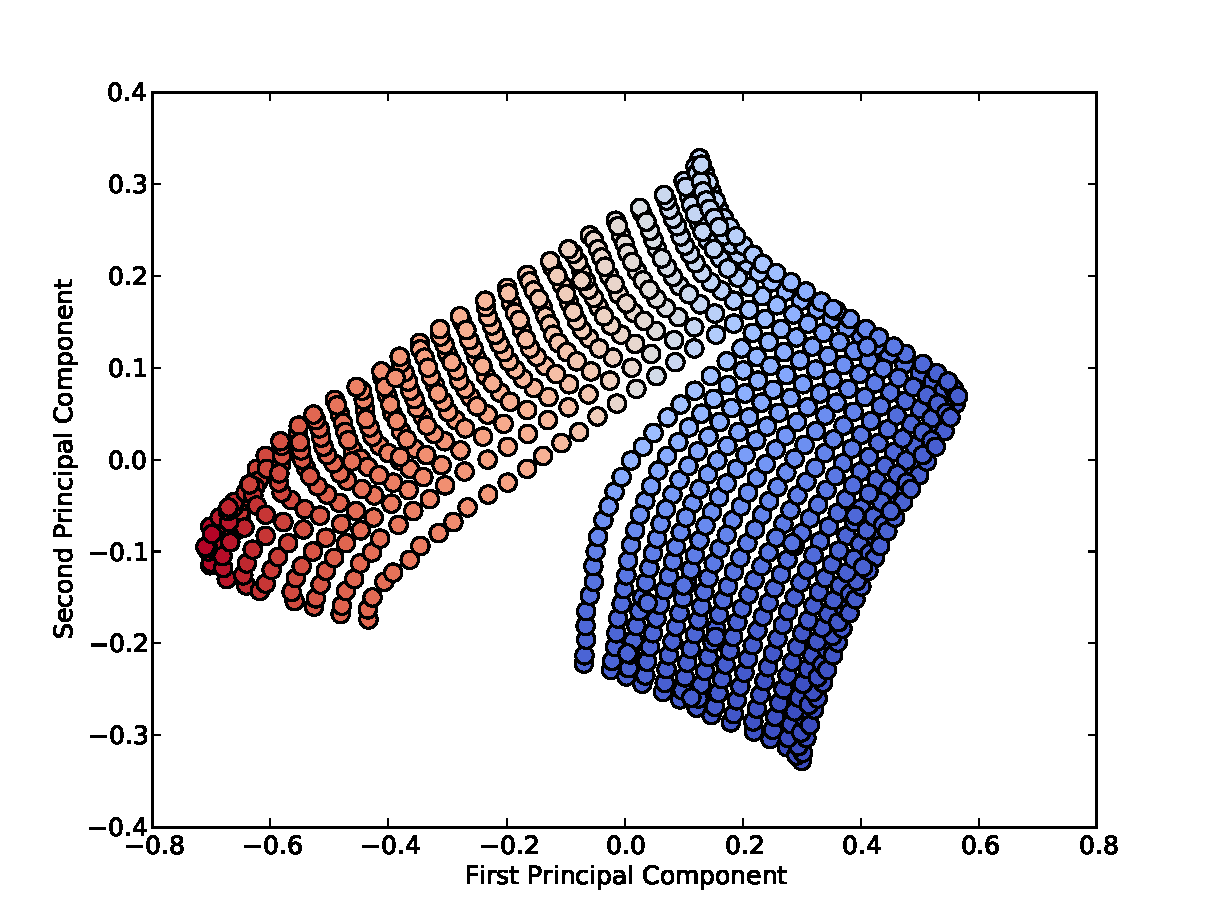
\includegraphics[width=\linewidth]{../writeup/figs/chap4/2rmop2.pdf}
  \endminipage
  \minipage{0.32\textwidth}
    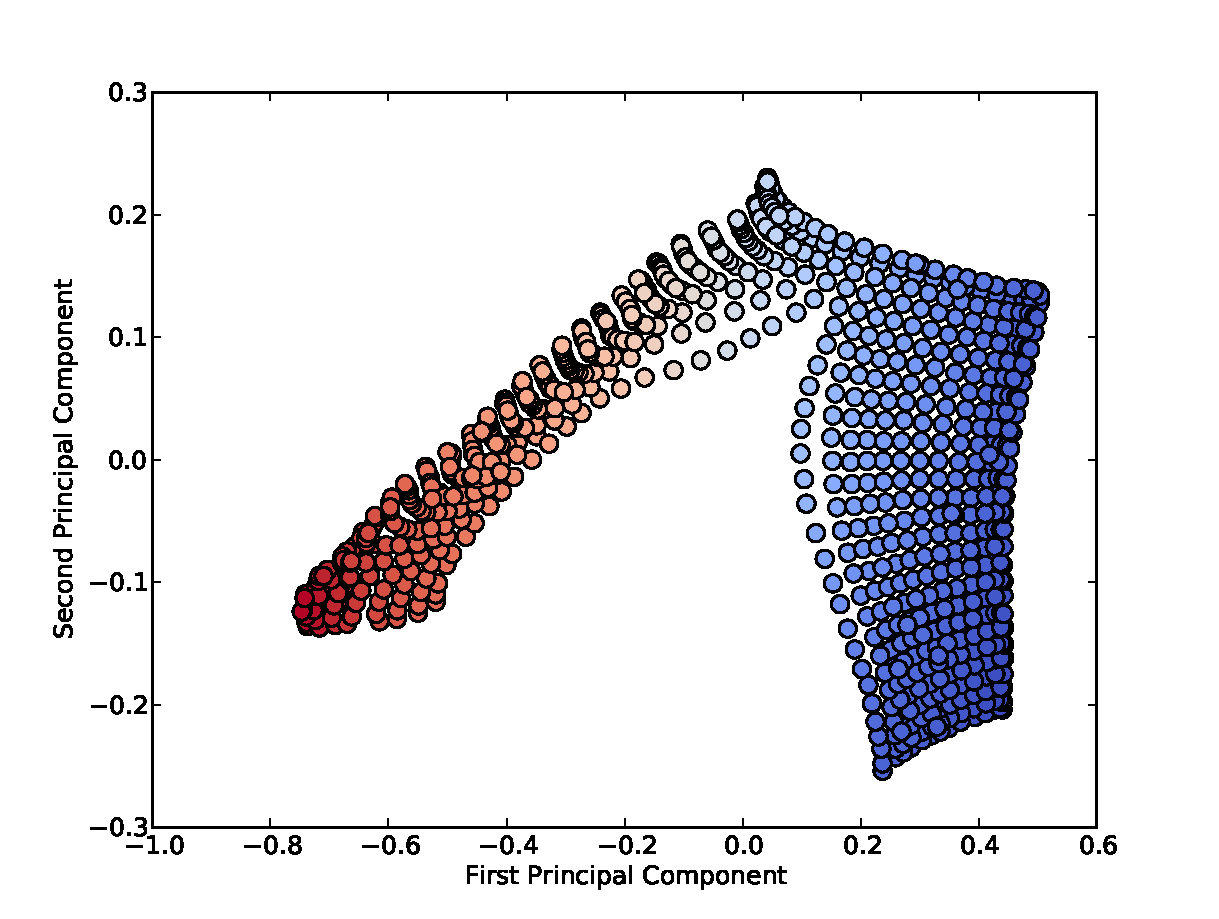
\includegraphics[width=\linewidth]{../writeup/figs/chap4/2rmop3.pdf}
  \endminipage
  \label{eyec}
\caption
{DKBRL opening the wall in \textit{TWO-ROOM} over three iterations.
Points are colored by ground truth value (red=high, blue=low).
After the first iteration (left) a rift has started to form, by the
third iteration points are completely separated by value.}
\end{figure}

\section{Results}

We start by demonstrating our approach work on Mountain-Car, a simple
reinforcement learning domain that allows us to easily
visualize the value function and gain insight about how DKBRL works.
We then present our main results:
performance improvements on the more challenging Acrobot and PinBall domains.

%\subsection{Experiment Formulation}
%We wanted the starts of our sample transitions to evenly cover the
%reachable state space.
%To estimate the reachable state space we performed several random walks
%starting from the start state.
%Once we established the reachable state space, we passed the points generated
%through a coverage filter to get the desired number of evenly spaced points.
%
%We used our own implementation of KBRL.
%It is similar to what is described by Ormoneit \& Sen \cite{kbrl},
%except our implementation creates a finite model that enforces the constraint
%that terminal states self transition with zero reward.
%We used a Gaussian as our mother kernel.
%Our implementation safeguards against arithmetic underflows by resorting to
%nearest neighbour whenever there is a divide by zero in the local averaging.
%The mother kernel used everywhere is a Gaussian.
%
%Our implementations of the three domains were adapted from code available on
%RL Glue \cite{rlglue}.
%The only major modifications we made was to normalize the domains to fit in
%a unit cell and to make the classes immutable as per our solver's API.

\subsection{Mountain-Car (proof-of-concept)}
Mountain-Car is a two dimensional MDP \cite{rlai}
modelling a car with a weak motor attempting to drive out of a valley.\footnote{
The code for Mountain-Car and Acrobot used for this paper was adapted from
RL-Glue \cite{rlglue}.}
The car is not powerful enough to escape directly and must build up
energy by rolling back and forth.
Mountain-Car's value function has a discontinuity that goes in a spiral through
the state space, separating states where the car has enough energy to make it
up the hill on its current roll from states that require an additional back
and forth.

\begin{figure}[!htb]
  \minipage{0.32\textwidth}
    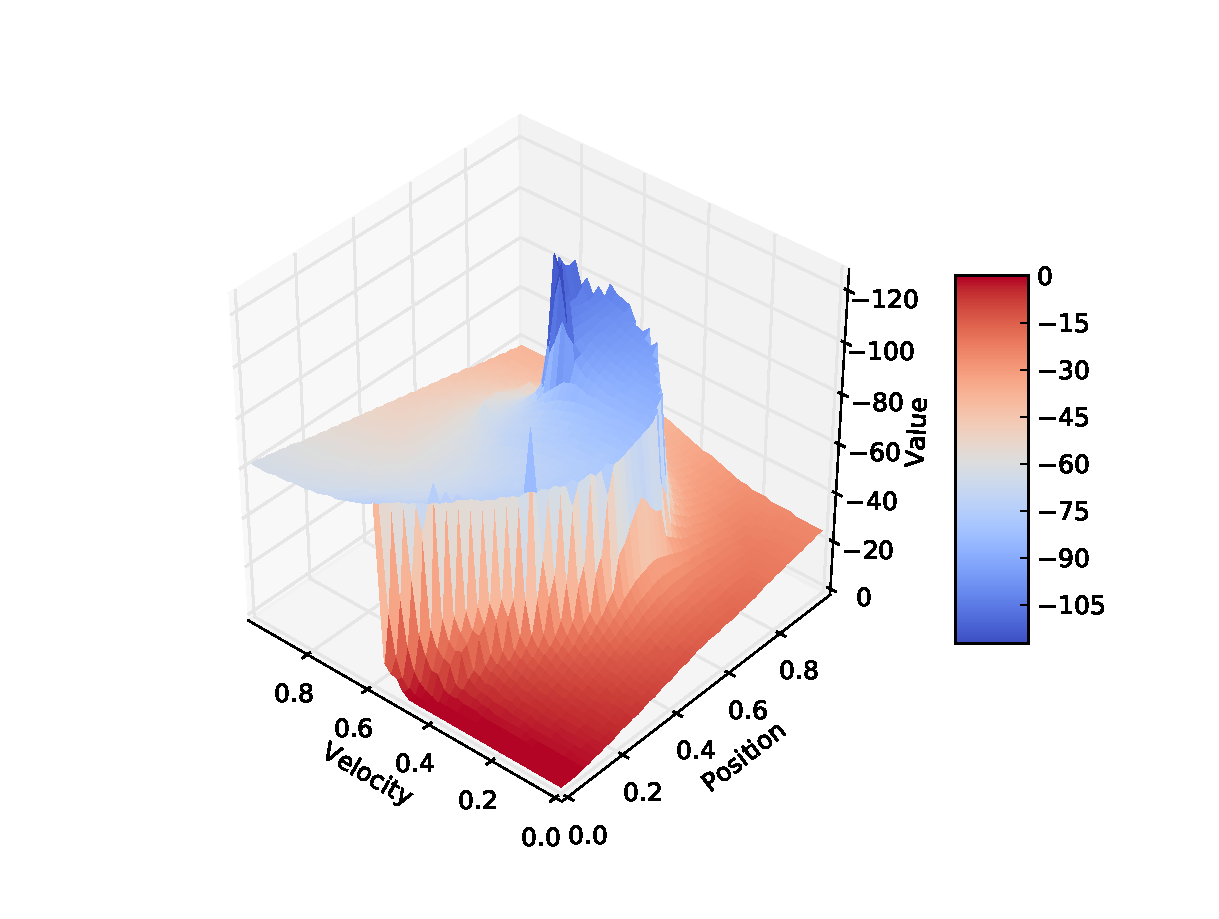
\includegraphics[width=\linewidth]{./figs/mctru.pdf}
  \endminipage
  \minipage{0.32\textwidth}
    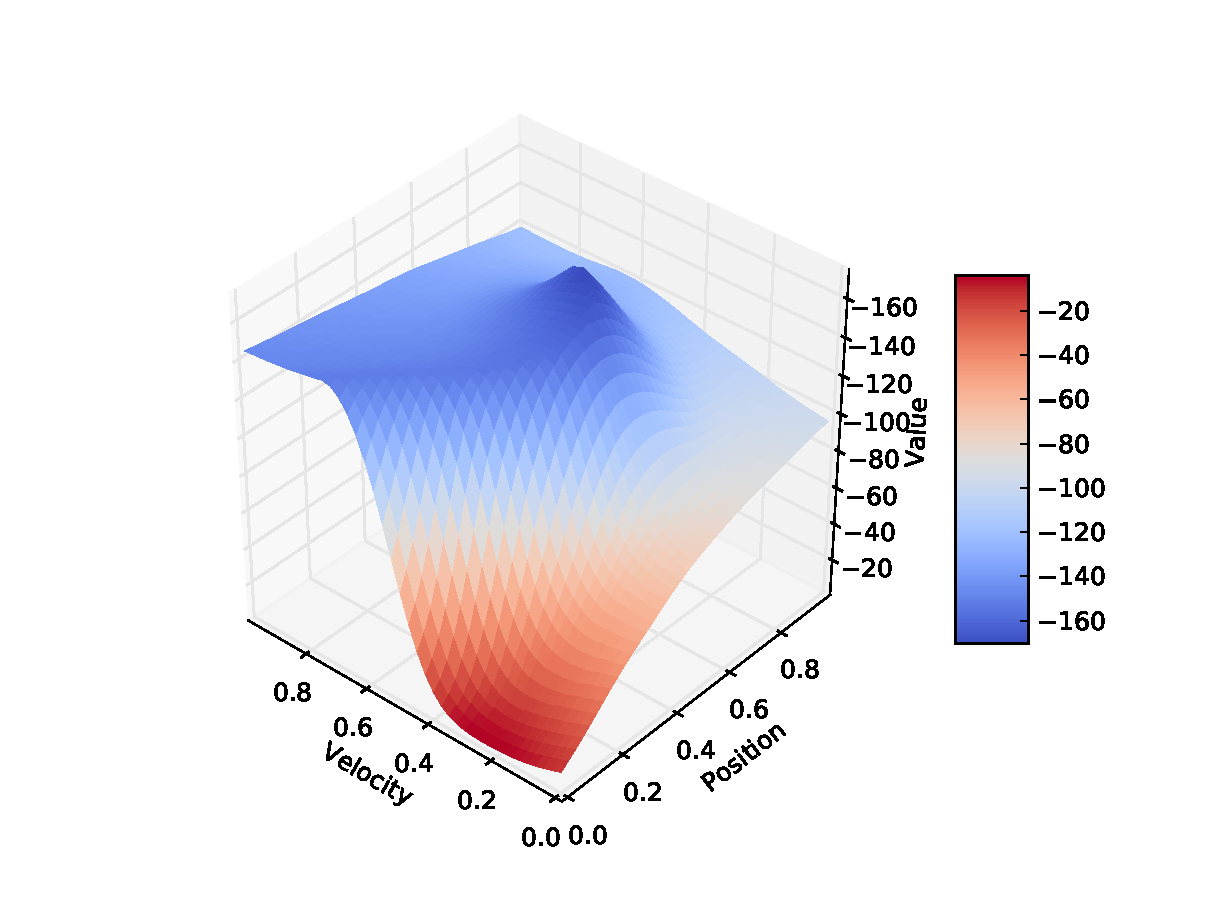
\includegraphics[width=\linewidth]{./figs/mc1.pdf}
  \endminipage\hfill
  \minipage{0.32\textwidth}
    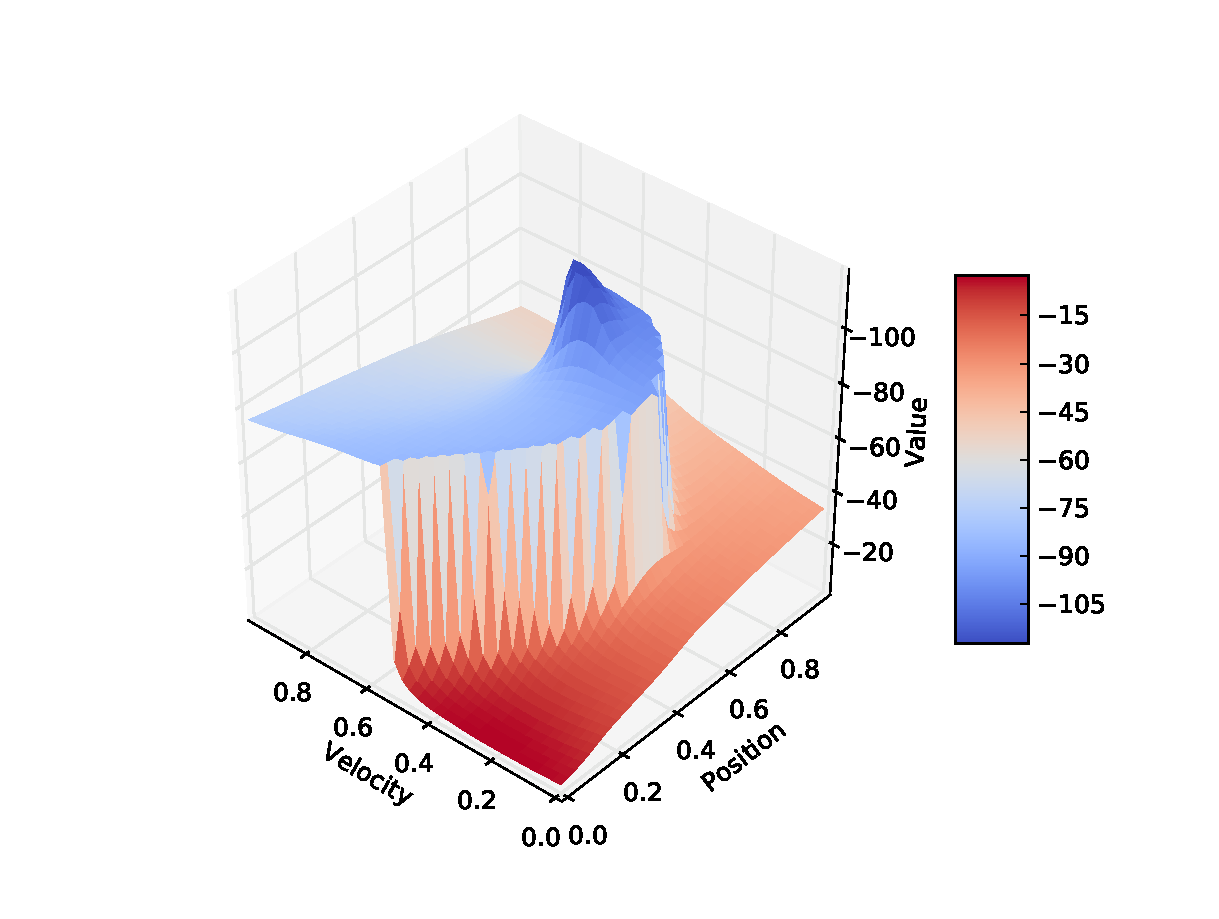
\includegraphics[width=\linewidth]{./figs/mc4.pdf}
  \endminipage
\caption{(Left to right) Mountain-Car's value function; the value function
as approximated by KBRL with $d_\mathrm{Euc}$ and $b=.09$; and
the approximation after four iterations of DKBRL with $\alpha=1$.}
\end{figure}

Our representation discovery algorithm allows KBRL to capture the discontinuity
remarkably well. It is also able to find the correct value for the bottom of the hill
(note the axes).
Nonetheless, because Mountain-Car is such an easy problem,
there is little difference in the policies induced by KBRL's and DKBRL's
value function approximations.
What matters for solution quality is not the value function approximation error, but
that the best action gets assigned the highest Q-Value.

\subsection{Acrobot}
Acrobot is a four-dimensional MDP \cite{rlai} modelling a two-link robot resembling a
gymnast on a high bar.
The gymnast can actuate at the waist and must raise its feet above some height by swinging
back and forth.
The acrobot domain has a value function discontinuity that resembles that of Mountain-Car.

For our experiments, we collected 15000 sample transitions per action, with start points
selected to uniformly cover the reachable state space.
We generated a solution from the transitions using KBRL then performed two iterations of DKBRL.
We conducted three sets of experiments, one for each bandwidth: $.03$, $.06$, and $.09$.
To account for the effects of random sampling we repeated each experiment 6 times and averaged
the results. For each run, we chose $\alpha = .5$ because that worked well in our regression experiments
in the supplementary materials.

\begin{figure}[!htb]
  \centering
  \minipage{0.3\textwidth}
    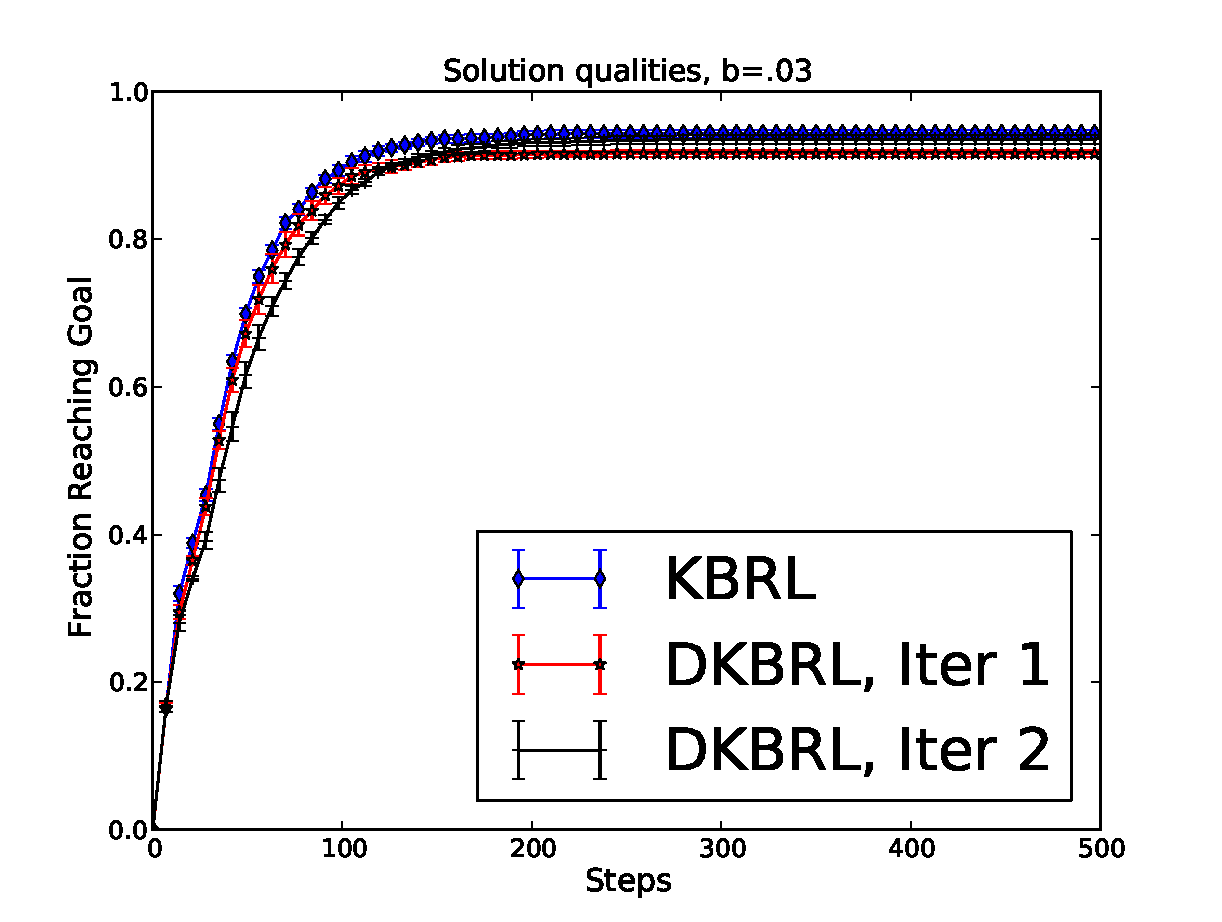
\includegraphics[width=\linewidth]{./figs/acb03.pdf}
  \endminipage\hfill
  \minipage{0.3\textwidth}
    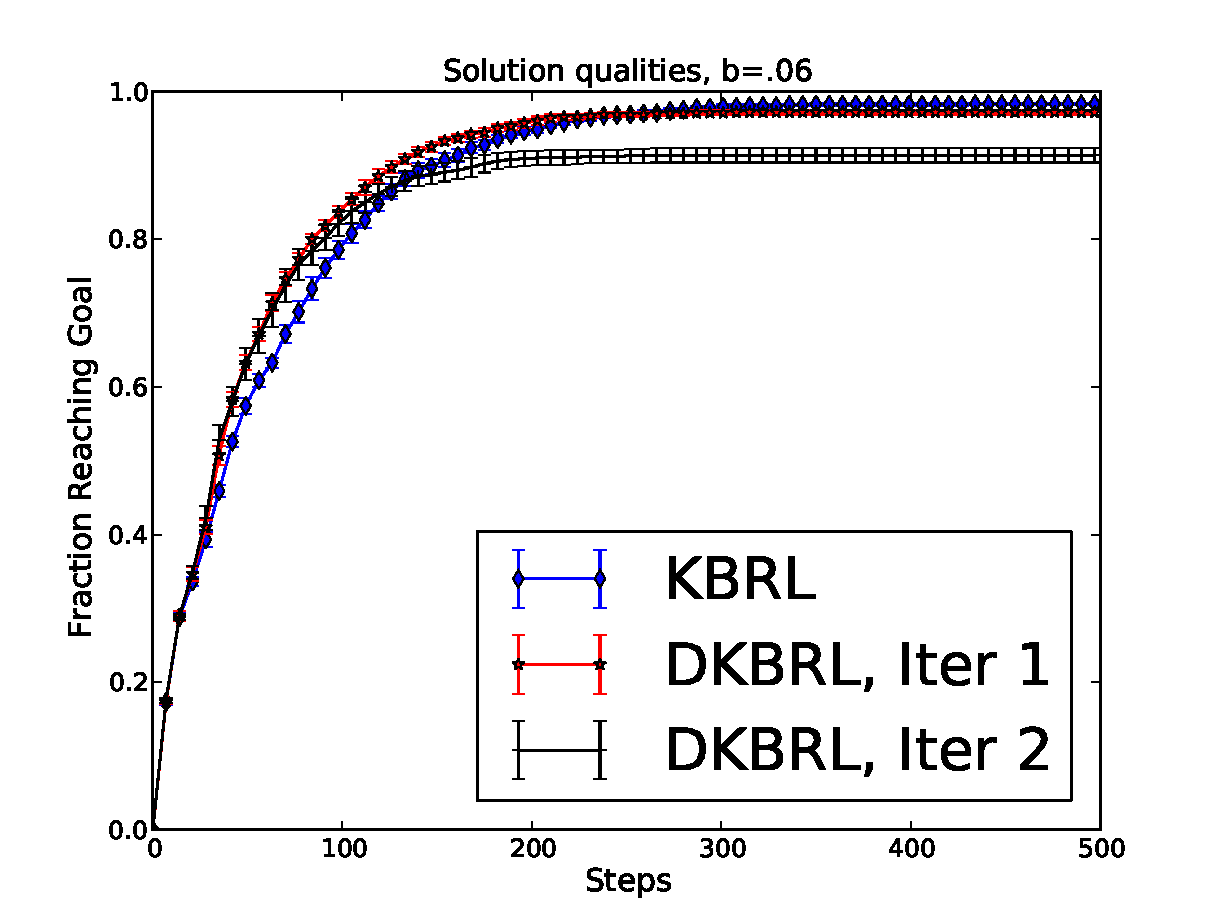
\includegraphics[width=\linewidth]{./figs/acb06.pdf}
  \endminipage\hfill
  \minipage{0.3\textwidth}
    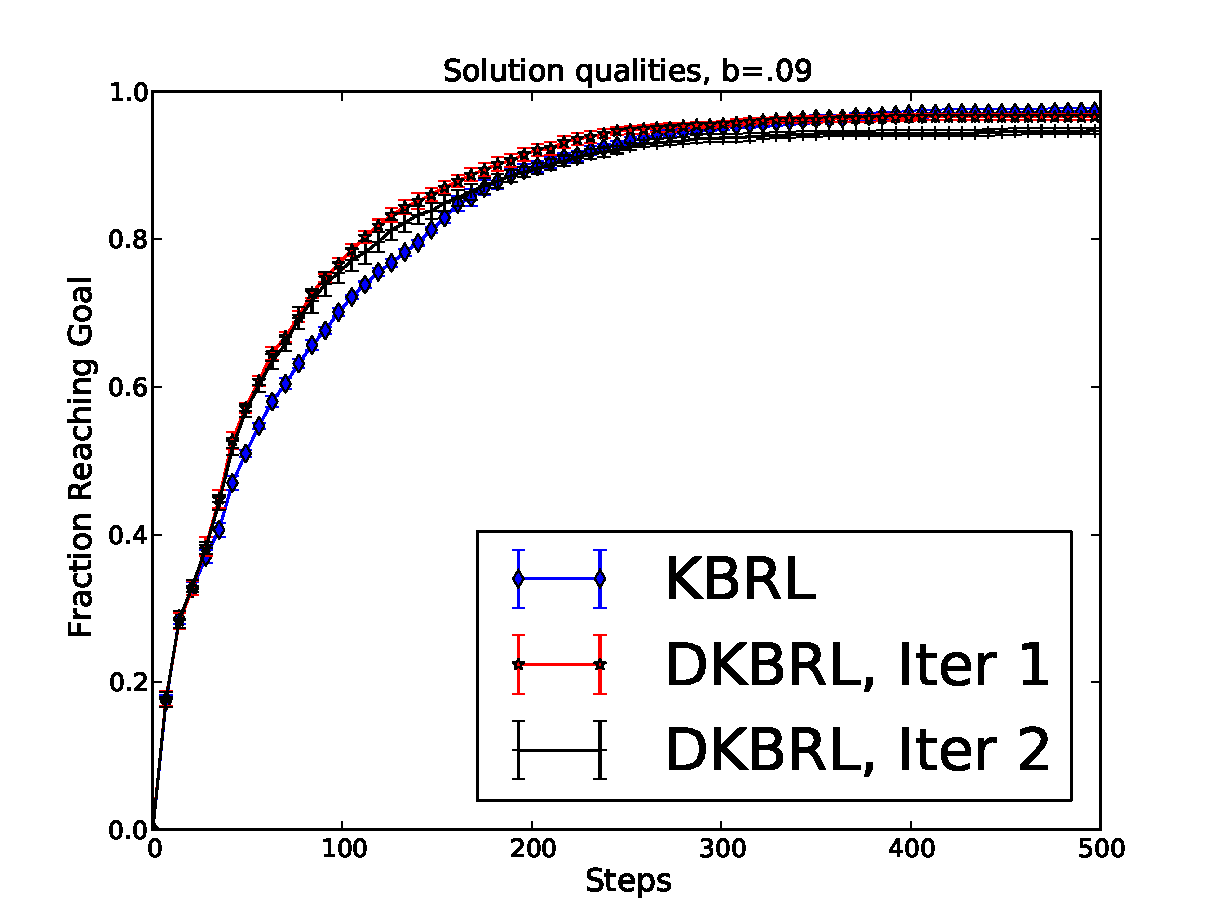
\includegraphics[width=\linewidth]{./figs/acb09.pdf}
  \endminipage\hfill
\caption{(Top to bottom) The average solution qualities for the three experiments.
The plots show the cumulative distributions of steps-to-goal.
The standard errors are drawn on the graph.}
\label{AcroFig}
\end{figure}

Figure \ref{AcroFig} shows the average solution qualities for the three sets of experiments.
Each plot shows cumulative distribution of the number of steps it took to reach the goal state
from ~230 start states selected to uniformly cover the reachable state space.
Note that the plots are the averages of the 6 experiments performed at each bandwidth
and that the standard-errors are drawn on the graph but are hard to see because they are so small.

We now point out the salient features of the graphs. 
In roughly 30\% of states, the agent is near the end of a trajectory
that reachs the goal (i.e. $<50$ steps from the goal).
In these easy states all the solutions perform the same.
The solution quality in the remaining 70\% of states is what matters.

For the size of our dataset, $b=.03$ is too small; KBRL undersmooths and produces a bad initial policy
that doesn't reach the goal for 5\% of states.
Performing DAWIT starting from this solution amplifies the noise and produces even worse policies.
When we chose the more reasonable $b=.06$, KBRL produces a good policy.
One round of DKBRL is able to improve on this, slightly shortening the steps-to-goal for
~65\% of all states.
The next round of DKBRL, however, is counter-productive, failing to reach the goal from 10\% of states.
When $b=.09$ the effects of oversmoothing the discontinuities starts to show for KBRL.
The graph is much slower to rise than when $b=.06$. A round of DKBRL offers a sizeable improvement
for  60\% of states. The second round of DKBRL offers no additional improvement.

Since DAWIT is designed to solve the problem of oversmoothing at discontinuities,
we would expect DKBRL to improve over KBRL when the bandwidth is large.
This is what appears to be happening here, but it is difficult to say for sure because the graphs
are so similar.
Because the discontinuity in Acrobot's value function is not along a decision boundary,
improving the fit there does not do much for solution quality.
In the next subsection, we consider a domain where discontinuities correspond to decision boundaries.

\subsection{PinBall}
PinBall is a four-dimensional MDP that models a ball navigating through a maze towards
a goal \cite{gdk}. The ball is dynamic, and bounces off obstacles;
the five actions allow the ball to either stay in place or accelerate slightly
along one of the compass directions.
PinBall is particularly challenging because it is easy to get stuck on a wall
while rounding a corner.
Furthermore, some of the obstacles are so thin that they are hard to detect
from the sample transitions.

We conducted our tests on one of the maps that came with the open source code.\footnote{
The code is available at \url{http://www-all.cs.umass.edu/~gdk/pinball/}. We used the map
\textit{pinball-easy.cfg}}
We had to make two modifications to the domain: first, we fixed a bug that
allowed the ball to pass through walls under some circumstances and second,
we increased the time discretization threefold so as to reduce the amount of data needed to solve
the problem.

For this set of experiments, we collected 20000 sample transitions per action uniformly from
the reachable state space. We then passed the samples through KBRL followed by two
iterations of DKBRL. We did this four times each at bandwidths $.04$, $.07$ and $.09$ keeping
the relaxation rate fixed at $\alpha=.5$.
The resulting steps-to-goal cumulative distributions are showin in Figure \ref{PbFig}.

\begin{figure}[!htb]
  \minipage{0.3\textwidth}
    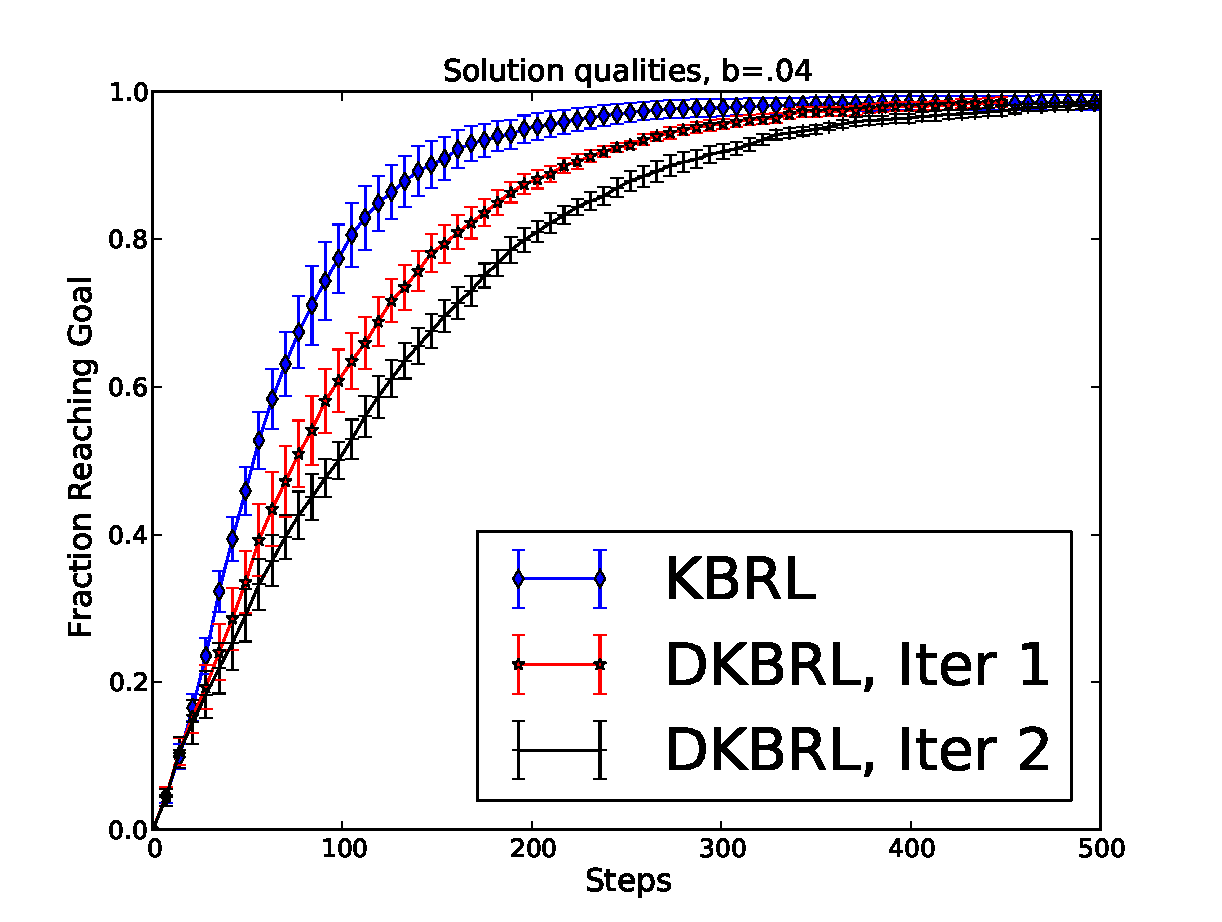
\includegraphics[width=\linewidth]{./figs/pb4.pdf}
  \endminipage
  \minipage{0.3\textwidth}
    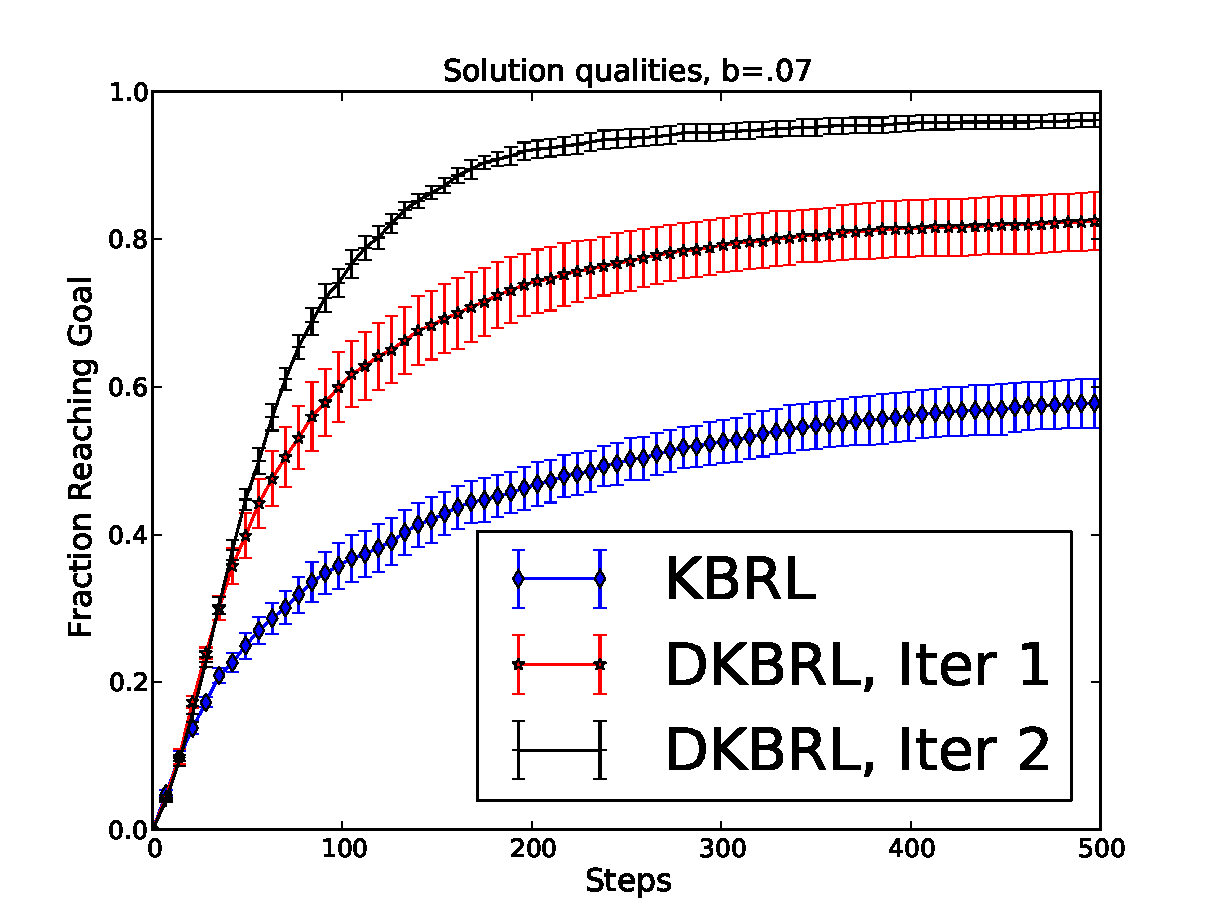
\includegraphics[width=\linewidth]{./figs/pb7.pdf}
  \endminipage
  \minipage{0.3\textwidth}
    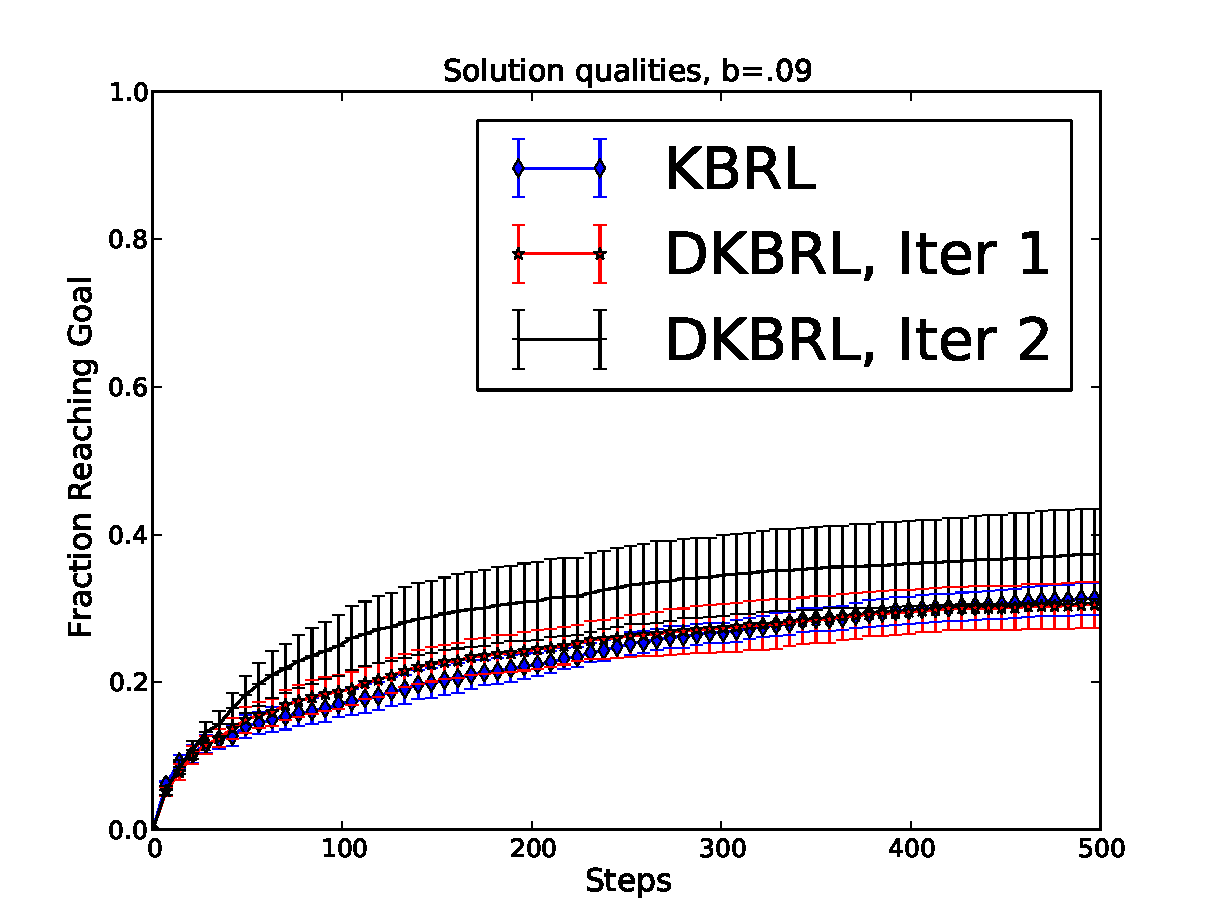
\includegraphics[width=\linewidth]{./figs/pb9.pdf}
  \endminipage
\caption{The average solution qualities for PinBall for $b=.04$, $.07$, and $.09$ respectively.}
\label{PbFig}
\end{figure}


For our chosen sample size, $b=.04$ is near the optimal value for KBRL.
KBRL produces its best solution there and performing iterations of DKBRL makes the performance worse.
We suspect that this happens because the value function approximation produced by
KBRL has large ripples\footnote{In our discussion of \textit{TWO-ROOM} we note that
performing KBRL with small bandwidths produces value functions with the right overall shape
but with ripples} which then get amplified by DAWIT making the fit worse.

When we raise the bandwidth to $b=.07$, the effects of oversmoothing kick in and the
performance of KBRL plummets. Here DKBRL is able to counteract the bias resulting from
oversmoothing and produce a solution comparable to the one produced by KBRL at $b=.04$.
The resulting average for the second iteration of DKBRL with $b=.07$ is similar to that of
KBRL with $b=.04$, but the variance is smaller.

Finally, when we raise the bandwidth to $.09$, the oversmoothing of KBRL is too much for DAWIT
to undo. DKBRL manages to improve upon the initial solution, but not by much.

These experiments suggest that the key merit of DKBRL is that it can reduce the need for bandwidth
tuning by allowing for near optimal solutions to be found over a wider interval of bandwidths.

\section{Related Work}

The method closest to ours for non-parametric regression is Metric Learning for Kernel Regression
(MLKR) \cite{mlkr},
which finds the Mahalanobis metric best suited for performing kernel regression.
Using Mahalanobis distance is equivalent to applying a linear transform to the input space.
Linear transforms are not powerful enough to smooth out discontinuities and would
offer little help approximating \textit{TWO-ROOM}'s value function. 
Predictive Projections \cite{sprague} uses an approach similar to MLKR for
dimensionality reduction in parametric reinforcement learning.

Other related algorithms are ST-ISOMAP \cite{jenkins} and Action Respecting
Embedding \cite{bowling}, which use modified nearest-neighbors algorithms to 
discover and unroll the manifold containing the data.
These algorithms have not been applied to RL.
They would be well suited for learning a representation for problems
where value function discontinuity arises from local state space topology.

Existing representation discovery algorithms for parametric RL have largely focused on
modifying the parametric representation of the value function itself. One early
approach was Proto-value functions (or PVFs) \cite{pvf}, which uses
nearest neighbors on the sample transitions to discover the manifold of the state space
and uses the eigenfunctions of the graph Laplacian as a basis for representing the value
function.
PVFs, along with the related diffusion wavelet approach \cite{wavelets},
focus on the topology on the state space and offer little additional leverage
when discontinuities arise from the MDPs reward structure.
Another parametric approach is the use of Bellman-error basis functions (BEBF) \cite{parr},
which are learned basis functions that represent 
the Bellman error in previous approximations.
BEBFs are similar in spirit to the technique we present in this paper; however,
they are used as basis functions in a linear value function approximation architecture.

We do not attempt to produce experimental results comparing our algorithm to any
of the techniques presented above.
They attempt to address problems that are related to, but distinct from,
what DAWIT is designed for and there is no meaningful comparison that can be made.

\section{Conclusion and Future Work}

Representation discovery, which has so far been investigated primarily in parametric
approaches to reinforcement learning,  is a promising area in the context of
nonparametric approaches.
A particularly interesting next step would be to explore
an online version of DKBRL to that samples new points for coverage
in the transformed space.
The correctness guarantees of KBRL require sampling points uniformly from the domain.
Sampling uniformly from our transformed domain is equivalent to concentrating samples
near value function discontinuities in the state space, which is desirable since that is where
the value function is hardest to represent.

\subsubsection*{Acknowledgments}

We would like to acknowledge the help of Leslie Kaelbling and
Tom\'{a}s Lozano-P\'{e}rez through every step of this project.
We would also like to thank Tommi Jaakkola for a conversation about
kernels.

\small{
\bibliographystyle{unsrt}
\bibliography{example_paper}
}

\appendix
\section{Transforming For Improved Fit}
This section provides a different interpretation of DAWIT, the metric learning
algorithm presented in Section 4.1.
We start by introducing Fit-Improving Iterative Representation Adjustment
(FIIRA), a function approximation framework under which DAWIT falls.
We then present an intuitive explanation of the rational behind DAWIT.

\subsection{Fit-Improving Iterative Representation Adjustment}
The problem statement of curve-fitting is as follows: given a set of training
points, $D = \{(x_i,y_i)\ |\ i = 1, \ldots, n\}$, of point-value pairs with
$y_i = f(x_i)$ for some function $f : X \to \mathbb{R}$,
produce a function $\tilde f$ to approximate $f$ well, for some measure of
approximation quality.

A regressor, $r$, is a procedure for creating fits from some space of
functions, $\mathcal{F}_r$.
If $f$ is not well approximated by any function in $\mathcal{F}_r$,
the fit generated by $r$ is guaranteed to be poor.
One way to fix to this problem is to transform the domain of $f$ and work in a
space where $f$ \textit{is} well approximated. Choosing such a transform
requires prior knowledge or assumptions about $f$.

Since we are not in a position to make assumptions about $f$,
we wish to infer a transform directly from the data.
Our idea for doing so, is to pass $D$ to the regressor,
then use the approximation produced to infer a transform $\Phi$ of the
domain $X$ such that $f$ on $\Phi(X)$ is better approximated by $\mathcal{F}_r$.
Algorithm 1 describes the framework for doing this.
The procedure takes as input a dataset, $D$; a regressor, $REGR$;
and a transform generator, $TF$.

\begin{algorithm}
\caption{Fit-Improving Iterative Representation Adjustment}\label{FIIRA}
\begin{algorithmic}[1]
\Procedure{FIIRA}{$D,\ REGR,\ TF$}
	\State $\Phi_0 \gets x \mapsto x$
          \Comment{Identity transform}
        \State $D_0 \gets D$
	\State $i \gets 0$
	\Repeat
		\State $\tilde f_{i+1} \gets REGR(D_i)$
                  \Comment{Perform regression}
		\State $\Phi_{i+1}\gets TF(\tilde f_{i+1}, D_i)$
                  \Comment{Produce transform}
                \State $D_{i+1} \gets \{(\Phi_{i+1}(x), y)\ |\ (x,y) \in D_{i}\}$
                  \Comment{Update the dataset}
		\State $i \gets i+1$
	\Until{$\tilde f_{i} \approx \tilde f_{i-1}}$
           \Comment{Or until best fit attained}
	\State \textbf{return} $x \mapsto \tilde f_{i}(\Phi_{i-1}(x))$
\EndProcedure
\end{algorithmic}
\end{algorithm}

A formal analysis of the properties of FIIRA
for a general regression scheme and transform generator
is outside the scope of this paper and is left for future work.
What follows is a discussion of FIIRA for the special
case where the regressor is a local-averaging kernel smoother
and the transform generator is DAWIT.

\subsection{Dimension-Adding Wrinkle-Ironing Transform}
In the paper we claim that the metric created by DAWIT corresponds to a
transform that warps the state space through a higher dimension.
We now elaborate on that.

Consider a transform generator that, given a function $f$ with domain $X$, 
returns a transform $\Phi$ which maps every $x \in X$ to $\langle x | f(x)\rangle$
(the bar represents concatenation).
$\Phi$ stretches $X$ into $d+1$ dimensions in a way that
pulls apart points that differ in value (See Figure 6).

\begin{figure}[!htb]
  \minipage{0.5\textwidth}
    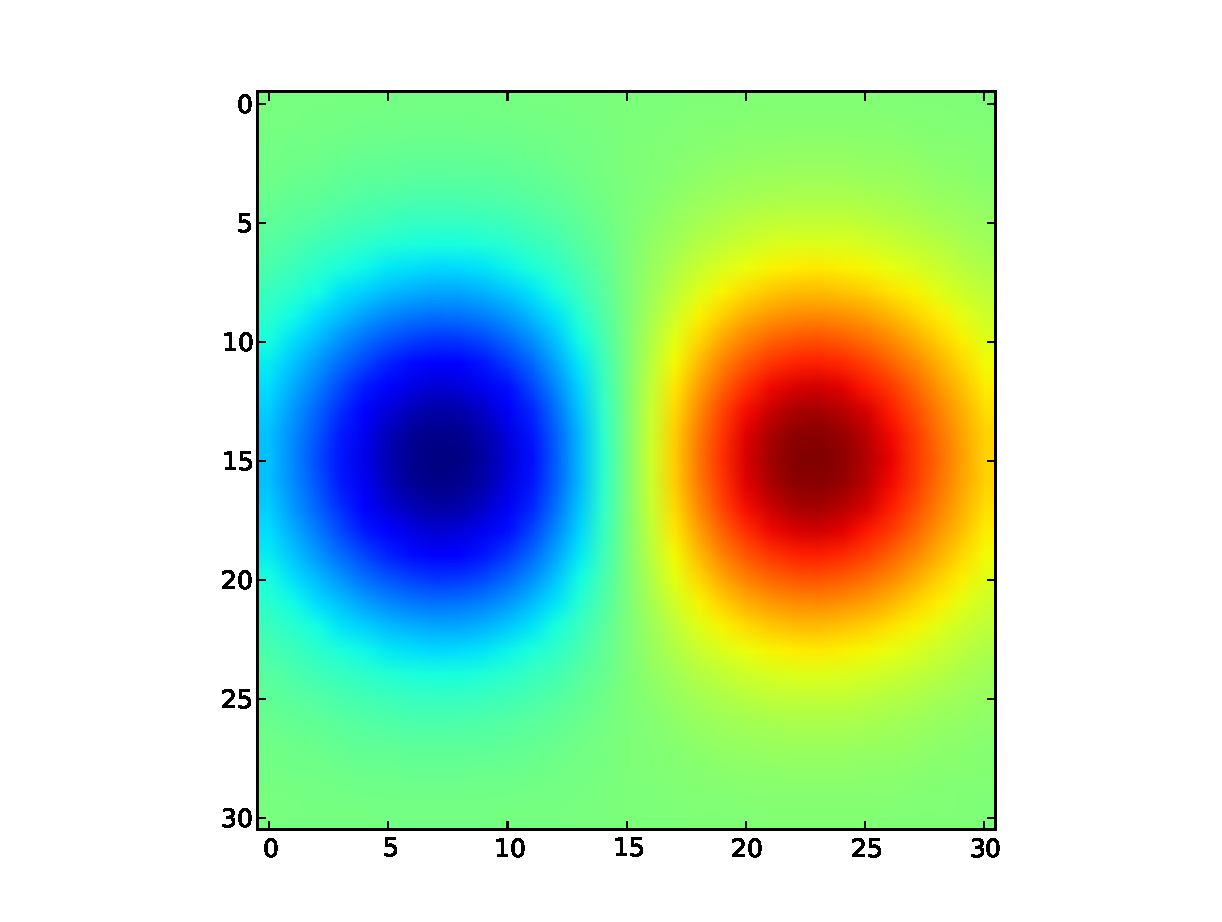
\includegraphics[width=\linewidth]{../writeup/figs/bumps.pdf}
  \endminipage\hfill
  \minipage{0.5\textwidth}
    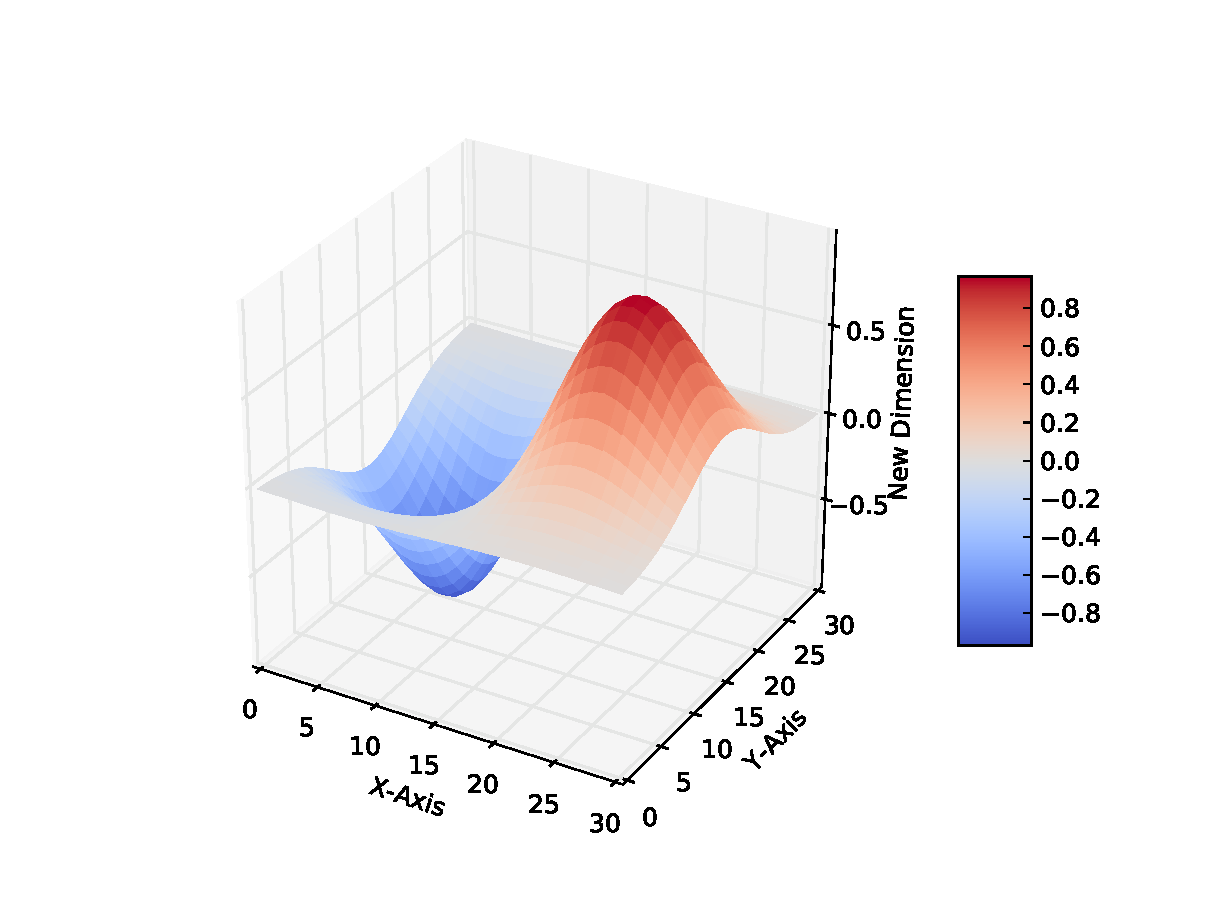
\includegraphics[width=\linewidth]{../writeup/figs/tfbumps.pdf}
  \endminipage
   \label{dimad}
\caption[Dimension-Adding WIT example]
{The figure on the left is a heatmap of some function with a two-dimensional
domain.
The areas in red are where it attains a high value and the ones in blue
are where it attains a low value.
The figure on the right shows the two-dimensional domain stretched through three
dimensional space in such a way that separates points that differ in value.
The red areas are pulled up and out of the page while the blue ones are pushed
down and into the page.
Distances in this transformed space correspond to the metric produced by DAWIT.}
\end{figure}

After the transformation, the distance between two points $a$ and $b$ in the
domain of $f$ becomes
$$\|\Phi(a)- \Phi(b)\| = \sqrt{\|a-b\|^2 + (f(a) - f(b))^2}.$$
Note that $\|\Phi(a)- \Phi(b)\|$ varies more closely with $|f(a) - f(b)|$
than does $\|a-b\|$.

The transform $\Phi$ does what we want, but it has two problems;
 it is sensitive to the scale of $f$, and it can change the diameter of $X$.
We fix these problems by normalizing $f$ by $\alpha\mu_f$ and $\Phi(X)$ by $c_0$
(as defined in the main body of the paper).

With these two changes, $\Phi$ maps the $m$-dimensional vector, $x = (x_1, \ldots, x_m)$
to the $m+1$-dimensional $x' = (c_0x_1, \ldots, c_0x_m, c_0\alpha\mu_f\cdot f(x))$.
The distance metric that corresponds to the final form of this transform is
 $$\|\Phi(a)- \Phi(b)\| = c_0 \sqrt{ \|a-b\|^2 + \alpha^2\mu_f^2\cdot(f(a) - f(b))^2}.$$
When we substitute for $\mu_f$ and $c_0$, this equals the metric produced by DAWIT;
hence the name ``dimension-adding'' VCPM relaxation.
We refer to kernel regression augmented to use DAWIT as FDK because it is a
\textbf{F}IIRA approach combining \textbf{D}AWIT and \textbf{K}ernel-regression.


\subsection{How DAWIT works}
Kernel-regression produces function estimates using local averaging.
As a result, the approximation is good where the target function, f,
is linear and bad where it has high curvature. It follows that the
curvature of the estimate, $h(x)$, is correlated with the approximation
error. Thus, we can infer where the approximation likely to be poor
just by looking at the approximation.

We use this insight to construct a transform of the input domain, $X$,
into a space where $h$ (and thus also $f$) are smoother. Our transform
warps the $m$ dimensional $X$ into the $m+1$ dimensional $X'$ in such a way
that its diameter is preserved but some neighborhoods grow or shrink
depending on the slope of $h$. The metric produced by DAWIT corresponds
to distances in $X'$.

Let $f$ be the unit step function and let $X = [-1,1]$. One iteration of
kernel regression produces $h$ resembling a sigmoid. $h$ attains its maximum
slope near $x=0$. Performing DAWIT with $h$ produces a metric, $d$, that
stretches the area around $x=0$ (i.e. $d(-\epsilon, \epsilon) > 2*\epsilon$,
for small $|\epsilon|$) and squashes the regions near $x=1$ and $x=-1$. The
point $x=0$ itself may get moved closer to $x=1$ or $x=-1$, but that
does not matter. What matters is that on the next round of regression
the region around $x=0$ is magnified, making it easier to pinpoint where
the discontinuity lies. This magnification is analogous to using a smaller bandwidth at $x=0$.

One can see now why we call the transform "wrinkle-ironing".
The discontinuity in the step function resembles a crease on an article of clothing.
Repeated application of the transform smooths this and similar value cliffs
much like a hot iron passing over a wrinkly shirt.

\subsection{Value Consistent Pseudometric}
In the main body of the paper, we claimed that using the VCPM as a valid
metric in kernel regression was theoretically sound. We now justify that claim.

When viewed under the lens of a FIIRA approach, the VCPM can be seen as coming
from a transform $\Phi^*$ that satisfies $\|\Phi^*(x)- \Phi^*(x')\| = \mu_f |f(x) - f(x')|$.
A transform that satisfies this property is $\Phi^*(x) = \mu_f f(x)$.
Under this interpretation, we are mapping each point to its scaled value
and performing kernel regression to fit a line.
Only points with identical values get mapped to the same point by the transform.
Since $\Phi^*$ is a safe to use before doing regression,
performing kernel regression with the VCMP for the function being approximated
cannot cause problems.

\clearpage

%\chapter{Proofs}
This section contains two proofs that were omitted from section 4.3.

\begin{claim}Any dataset $D = \{(x_1, y_1), (x_2, y_2)\}$ with $x_1 \neq x_2$
and $y_1 \neq y_2$ is a stable fixed point of FDK for any choice of kernel if
the
domain is taken to be the set $\{x_1, x_2\}$ (i.e. no
interpolation between the two points).\end{claim}

\begin{proof}The diameter of the domain is $\|x_1 - x_2\|$. Since
\textit{DAWIT} is diameter preserving, the two points in the domain do not
move relative to each other after the transformation.
It follows that $\|\Phi(x_1) - \Phi(x_2)\| = \|x_1 - x_2\|$ and thus
$\tilde f_1(x) = \tilde f_2(\Phi_1(x))$ for both $x_1$ and
$x_2$, making $D$ a fixed point of FDK.
Note that $D$ is not an attractive fixed point: if the
$x_i$ are perturbed, the result is a new fixed point.\end{proof}

\begin{claim}When done using a kernel, $k$, with compact support having
bandwidth,
$b < \frac{\mathrm{diam}(X)}{c}$ for some integer, $c$, FDK has a stable, attractive fixed point with
$c + 1$ atoms.\end{claim}

\begin{proof}(by construction)
Consider the dataset $D = \{(x_i,y_i)\ |\ i = 0\ldots c\}$ with $x_i = y_i = ic$.
We show that performing a round of FDK does not move the $x_i$ relative to
eachother, making $D$ a fixed point.

Solving for $\tilde f_0$ gives $$\tilde f_0(x) = \sum_i k(x,x_i)y_i = y_i.$$
Note that the value predicted for each $x_i$ is independent of $x_j\ \forall
j\neq i$. This is because a kernel centered on one point does not reach any
of the others.
Further note that $\tilde f_0$ is a line, making $D$ a fixed point 

To show that $D$ is an attractive fixed point, purturb every $x_i$ in the
domain by some $\epsilon_i$, setting $x_i' = x_i + \epsilon_i$.
If each $|\epsilon_i| < \frac{\mathrm{diam}(X)}{c} - b$,
it will still be the case that $\tilde f(x_i') = y_i$.
To straigten out $\tilde f$, the WIT will push each $x_i'$ closer to $x_i$.
This makes $D$ an attractive fixed point.
\end{proof}

The proof above shows that as the bandwidth shrinks, the number of atoms
increases.
This implies that the piecewise flat approximations generated with a
smaller bandwidth will have more pieces.
The proof can be extended to deal with kernels without compact support.

\clearpage
\newpage

\section{Graphs}
This section contains graphical demonstrations of the convergence
properties of FDK. It starts by showing how FDK converges to
a piecewise flat approximation when modelling a line.
It goes on to show the FDK fits generated for some datasets.

\begin{figure}[!htb]
  \minipage{0.3\textwidth}
    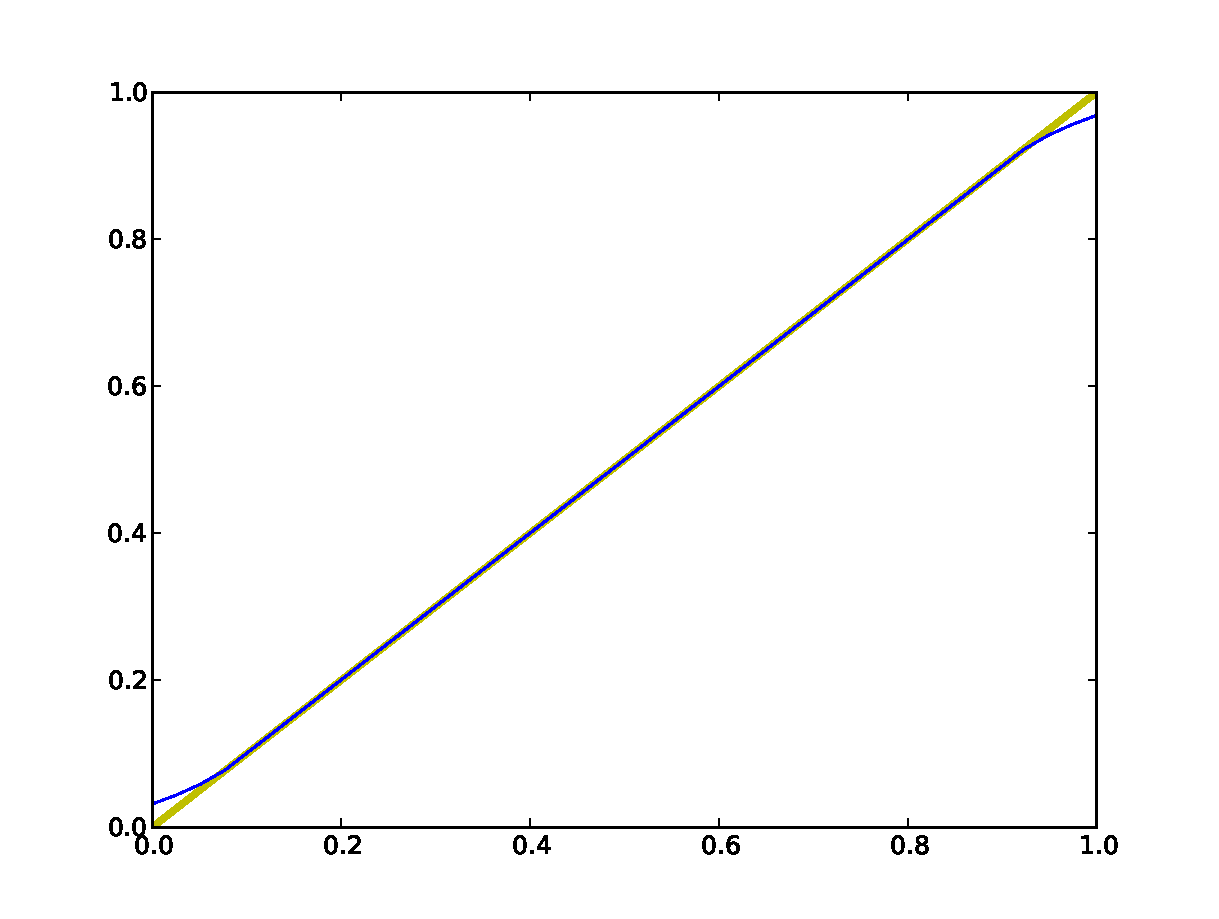
\includegraphics[width=\linewidth]{../writeup/figs/linefit.pdf}
  \endminipage\hfill
  \minipage{0.3\textwidth}
    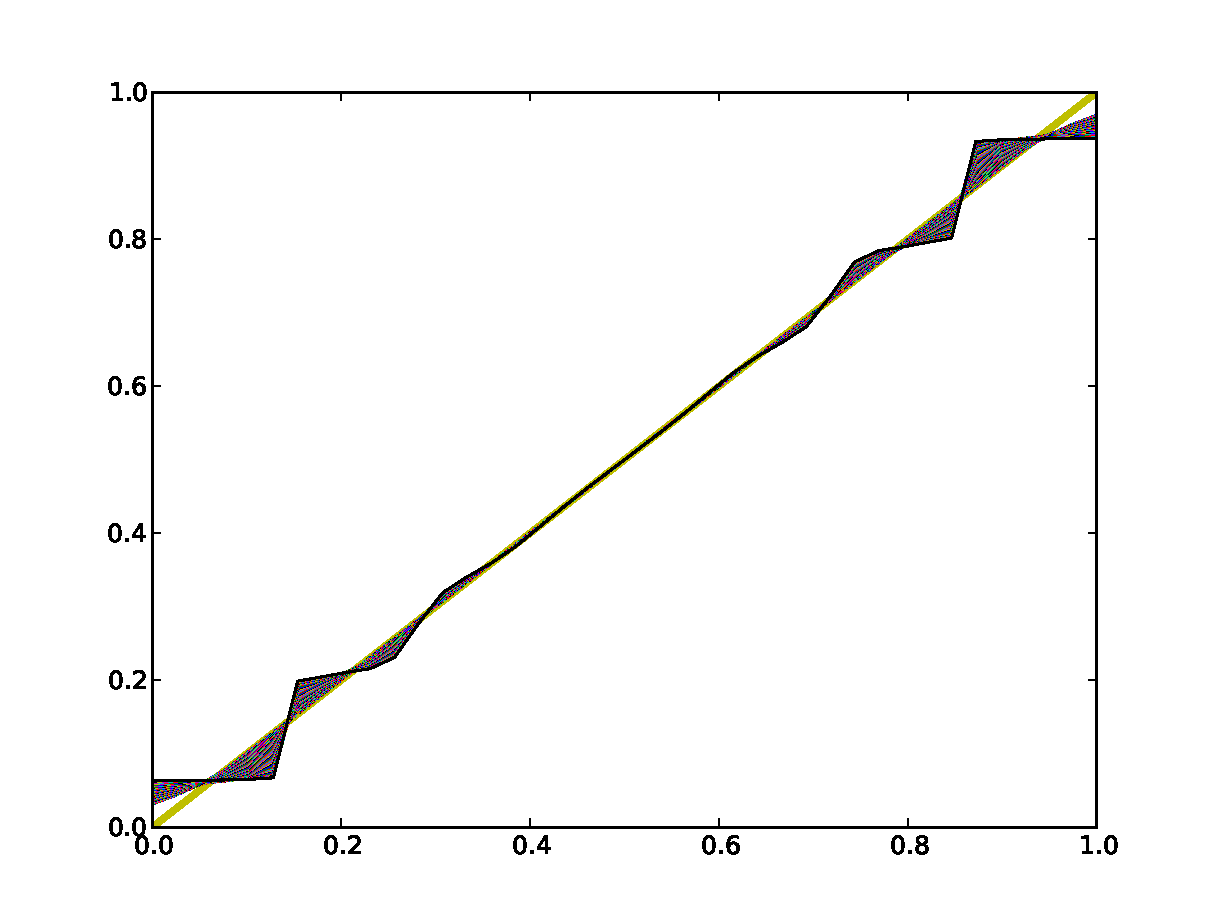
\includegraphics[width=\linewidth]{../writeup/figs/linefitmid.pdf}
  \endminipage\hfill
  \minipage{0.3\textwidth}
    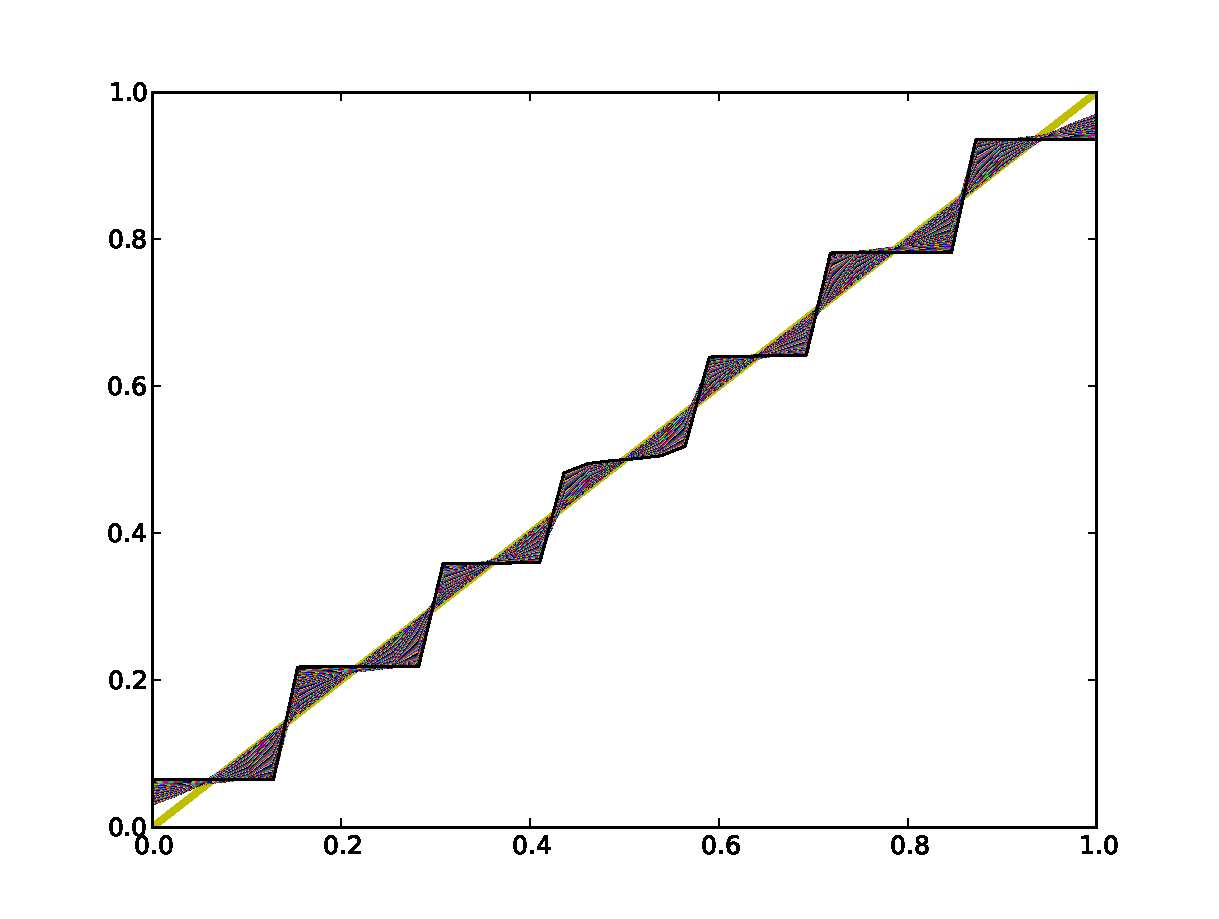
\includegraphics[width=\linewidth]{../writeup/figs/linefitend.pdf}
  \endminipage\hfill
\caption[Fitting a line]{How FDK converges to a piecewise flat approximation
when attempting to fit a line. The figure on the left shows the first fit
$\tilde f_0$ in blue. Note how the fit is biased at the boundaries.
This bias gets amplified over the next several iterations of FDK (middle).
The end result is the piecewise flat approximation on the right.
If we had used a smaller bandwidth there would have been more pieces
in the piecewise flat approximation.}
\end{figure}


When fitting a line, the approximation error increases with every iteration.
For most functions, however, the error goes down for a few iterations before going up.
The following figures show the result fitting some select functions with
different combinations of parameters.

Below we have included plots that show approximation quality of FDK for some
select datasets.
The plots on the left show the dataset (scatter plot), the kernel
regression fit (dotted blue line), the best FDK fit obtained (solid red line), and the
piecewise flat function to which FDK converges for the value of $\alpha$
that produced the best fit (green pluses).
The plots on the right show how the approximation error changes as a function of
iteration number for different values of $\alpha$.
Approximation error is measured as the sum of squared errors, normalized so that the fit produced
by the vanilla kernel regression has unit error. Note how low the error dips and how
few iterations it takes to get there.

\begin{figure}[!htb]
  \minipage{0.46\textwidth}
    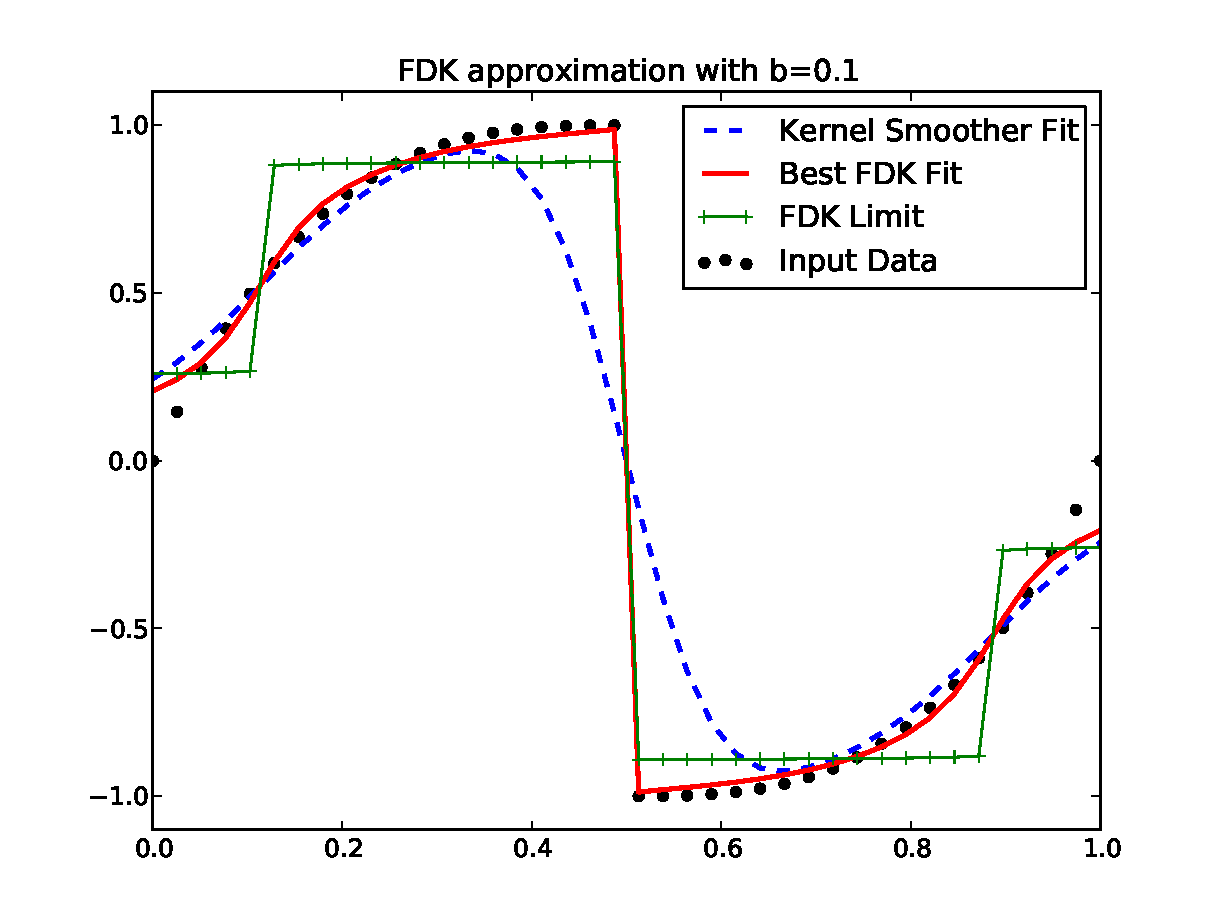
\includegraphics[width=\linewidth]{./figs/flip.pdf}
  \endminipage\hfill
  \minipage{0.46\textwidth}
    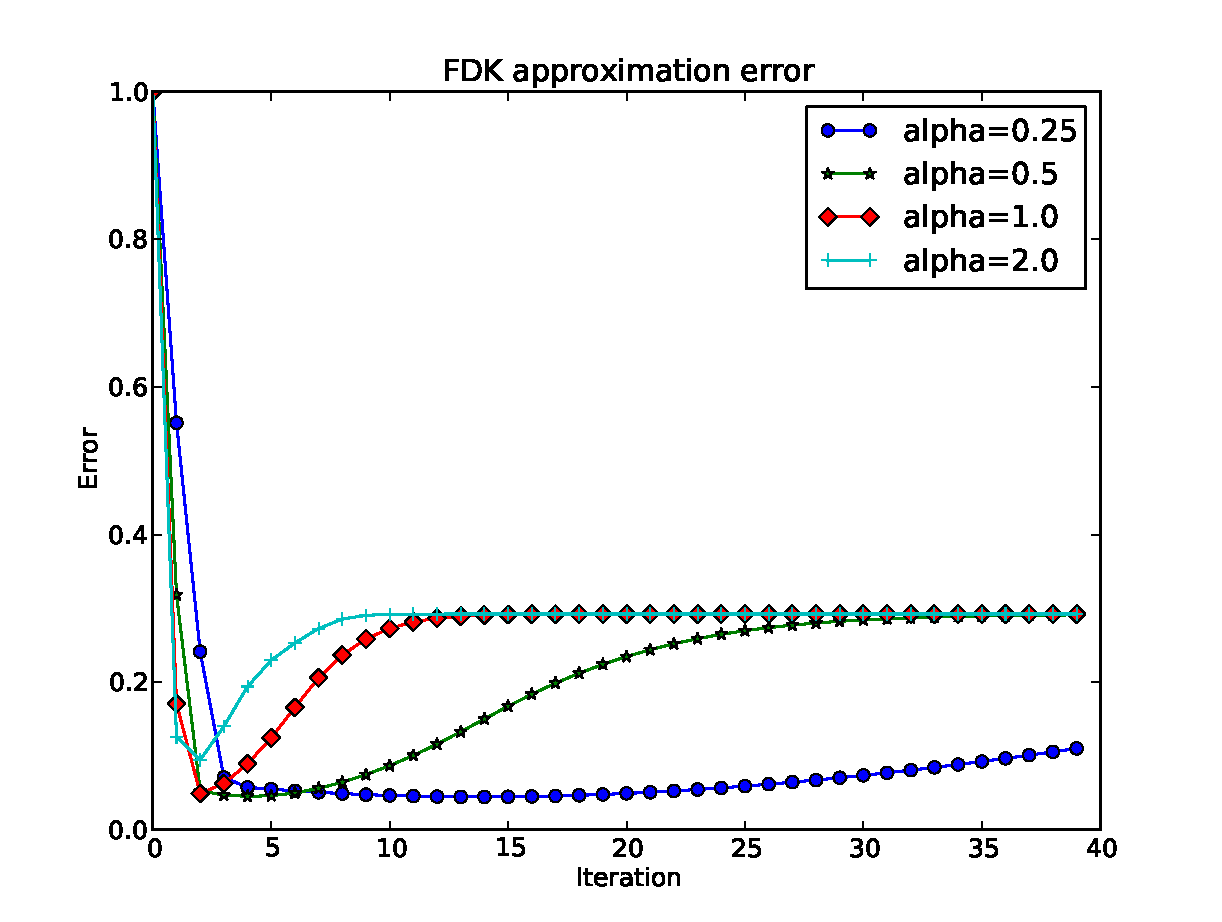
\includegraphics[width=\linewidth]{./figs/fliperr.pdf}
  \endminipage
%\caption[Fitting $x^3 - \mathrm{signum}(x)$]
%{FDK fit for $x^3 - \mathrm{signum}(x)$}
\end{figure}

\begin{figure}[!htb]
  \minipage{0.46\textwidth}
    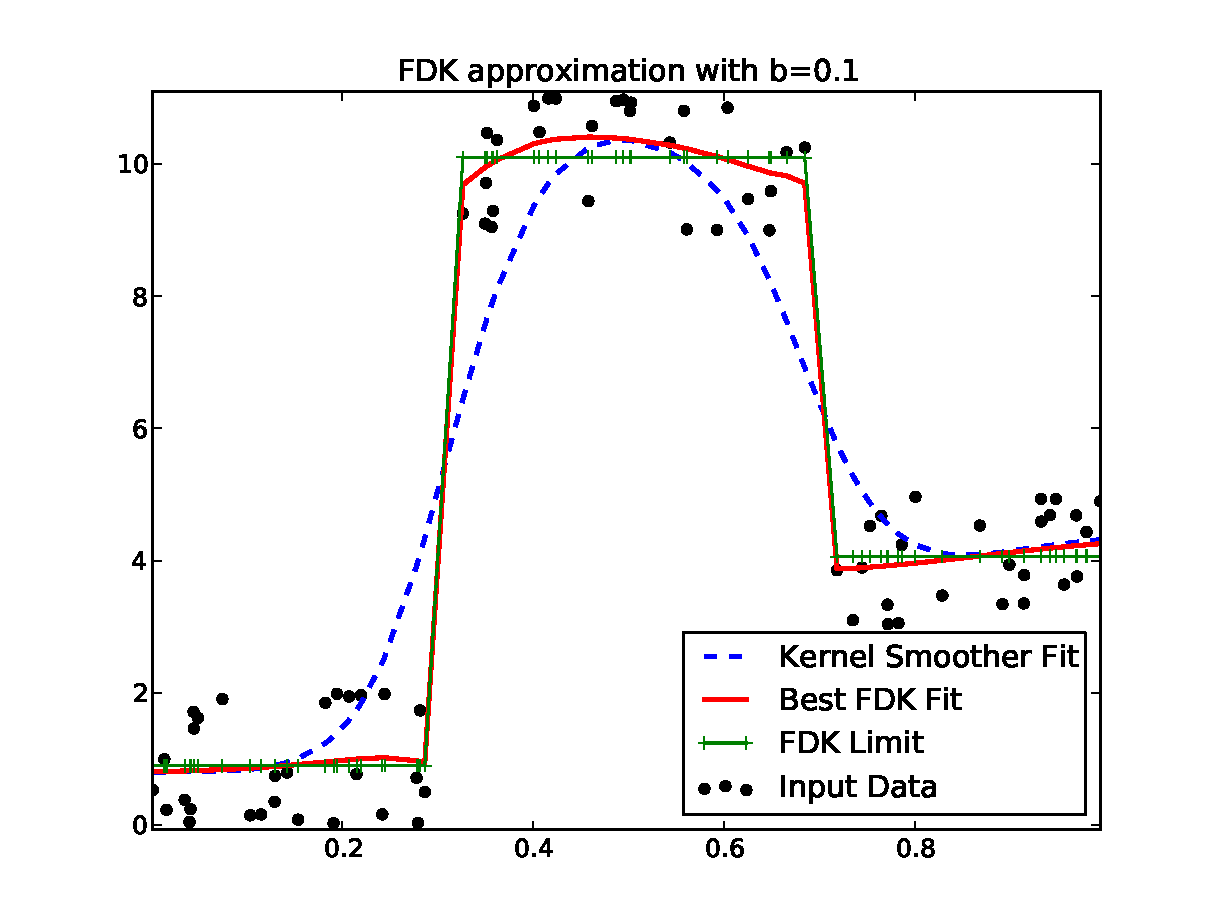
\includegraphics[width=\linewidth]{./figs/3step.pdf}
  \endminipage\hfill
  \minipage{0.46\textwidth}
    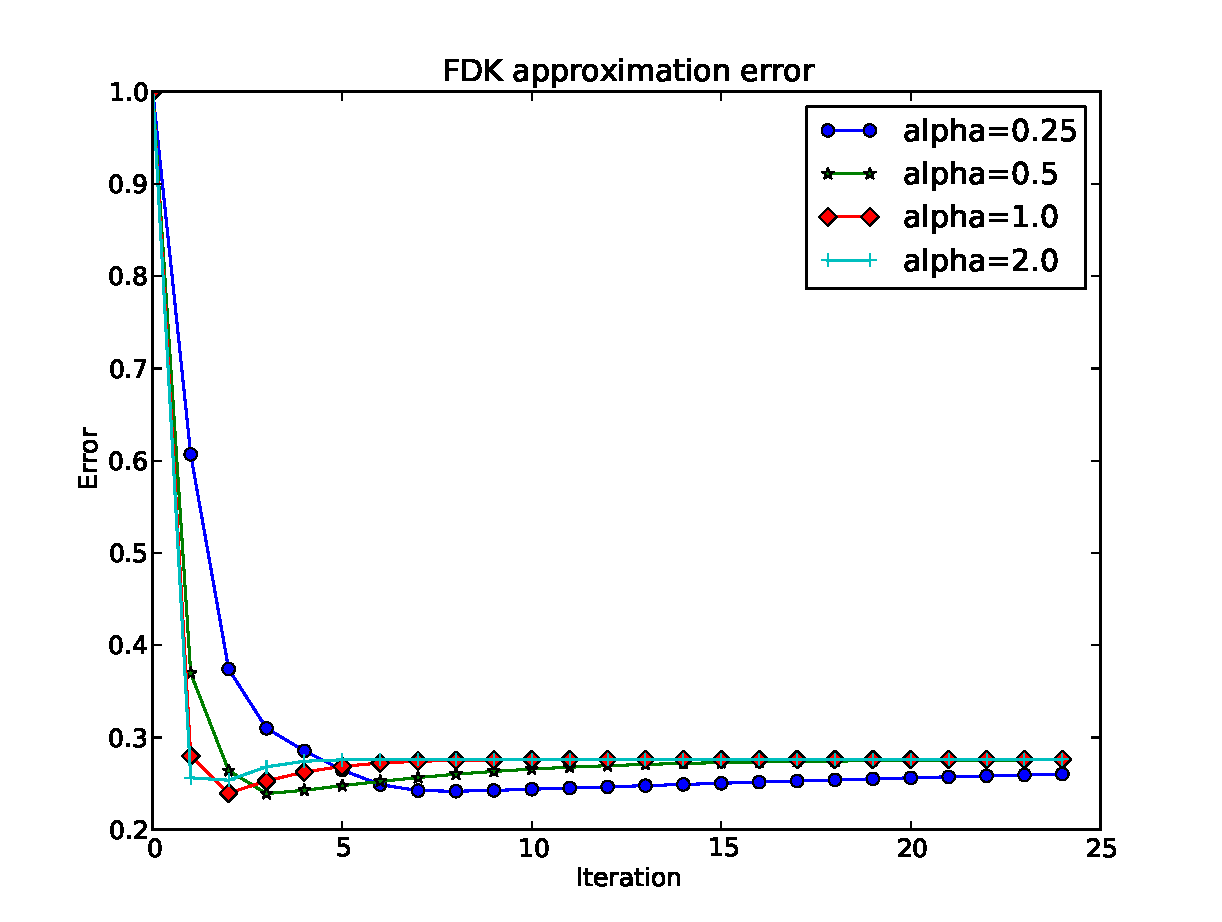
\includegraphics[width=\linewidth]{./figs/3steperr.pdf}
  \endminipage
%\caption[Fitting an order 5 Fourier function with $b = .25$]
%{FDK fit for the Fourier function above, this time with a larger bandwidth.}
\end{figure}

\begin{figure}[!htb]
  \minipage{0.46\textwidth}
    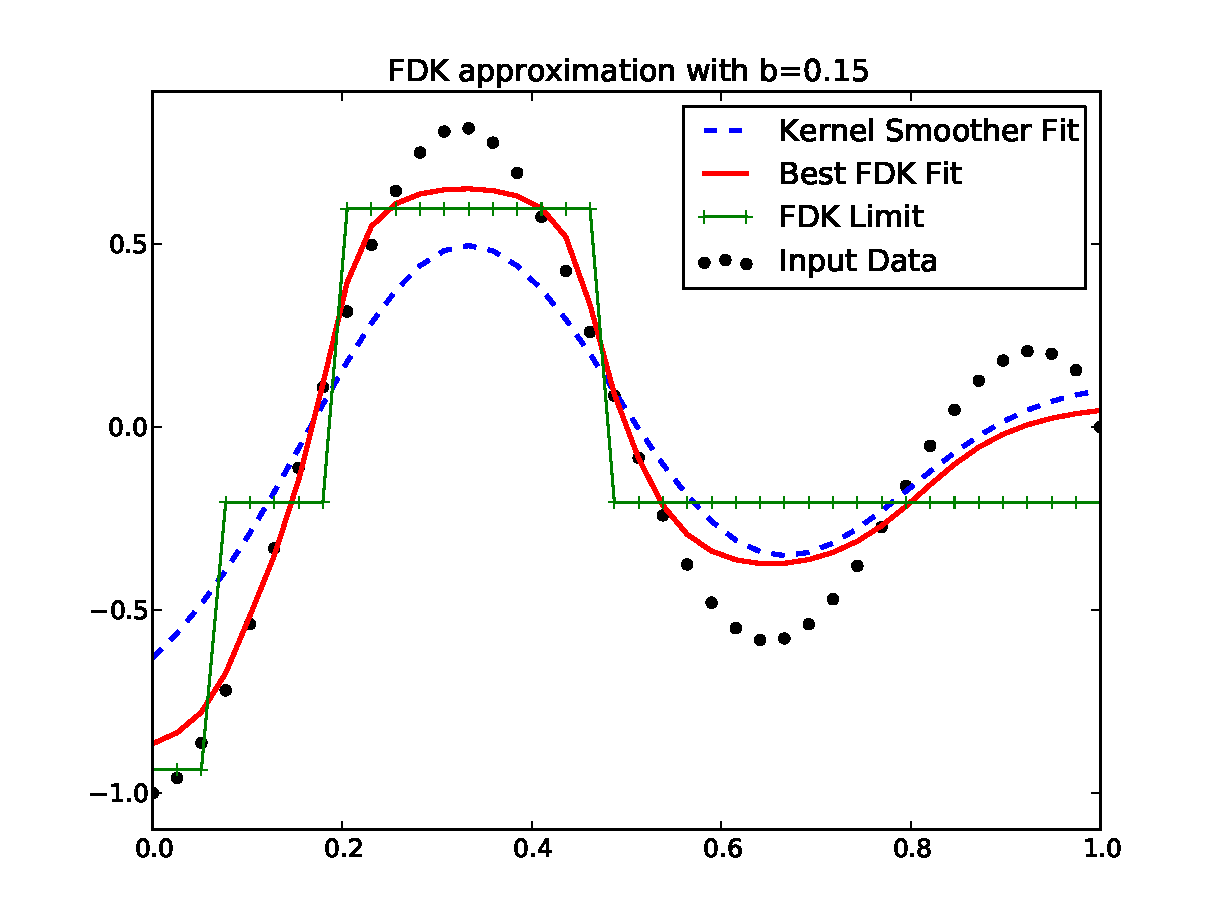
\includegraphics[width=\linewidth]{./figs/sqrtxcosx.pdf}
  \endminipage\hfill
  \minipage{0.46\textwidth}
    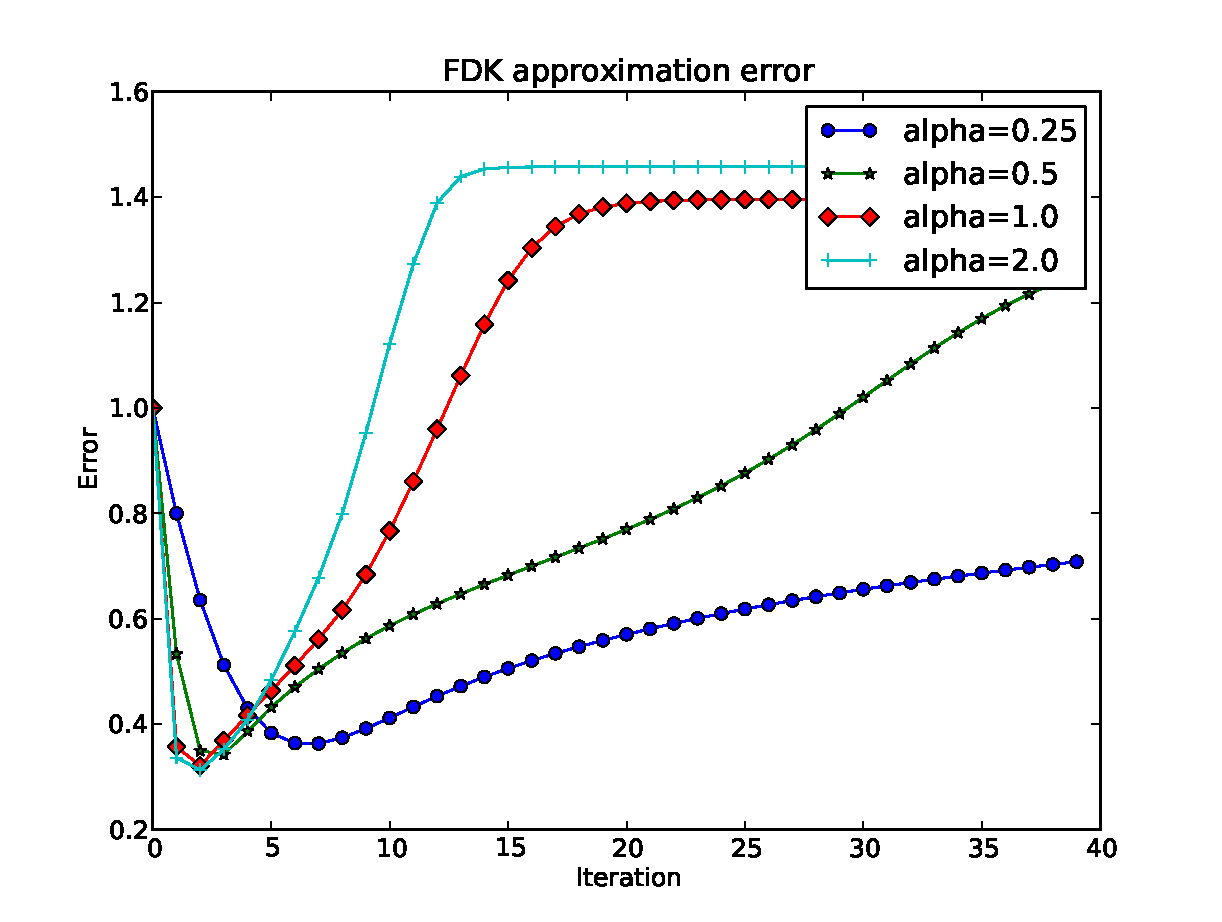
\includegraphics[width=\linewidth]{./figs/sqrtxcosxerr.pdf}
  \endminipage
%\caption[Fitting $-\sqrt{1-x}\cdot\mathrm{cos}(\pi x)$]
%{FDK fit for $-\sqrt{1-x}\cdot\mathrm{cos}(\pi x)$.}
\end{figure}

\begin{figure}[!htb]
  \minipage{0.46\textwidth}
    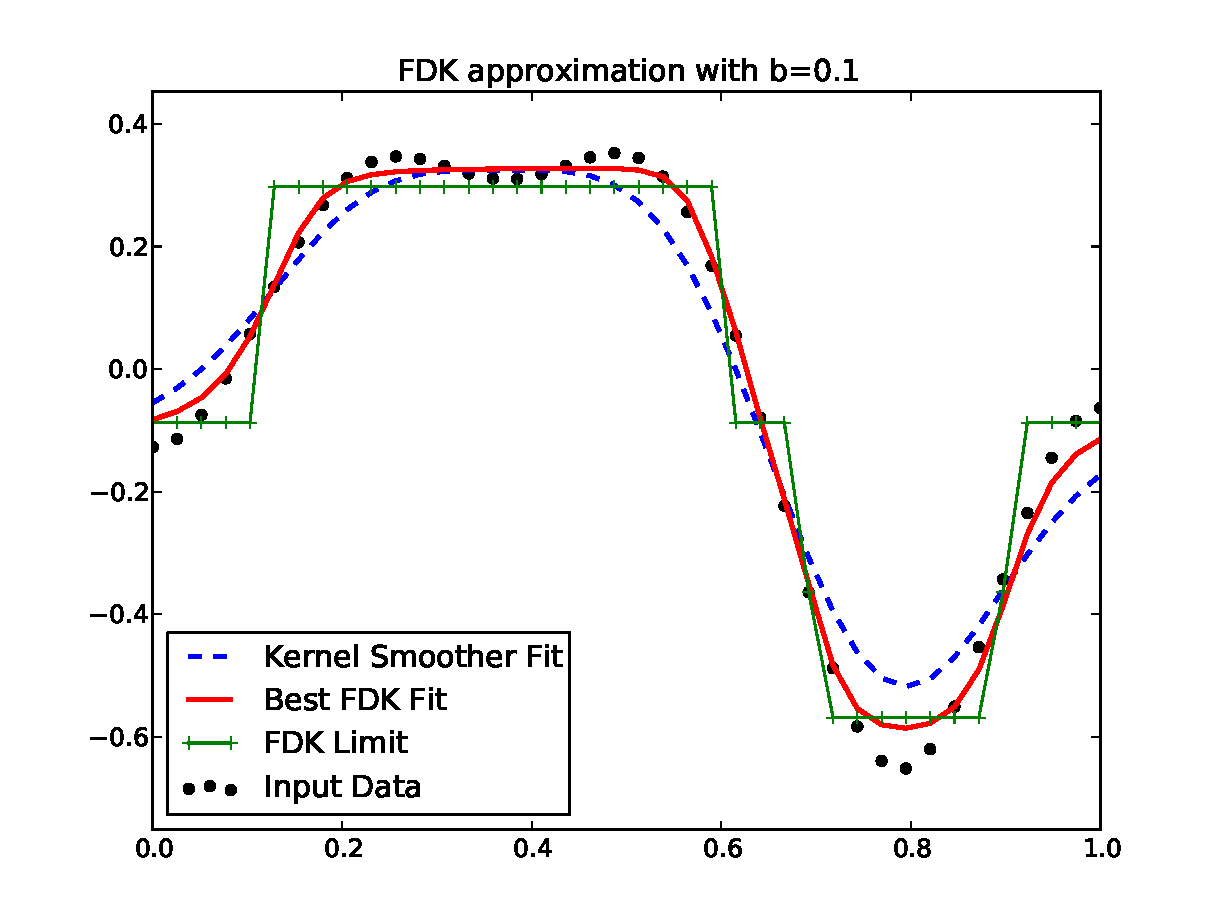
\includegraphics[width=\linewidth]{./figs/bumpy1.pdf}
  \endminipage\hfill
  \minipage{0.46\textwidth}
    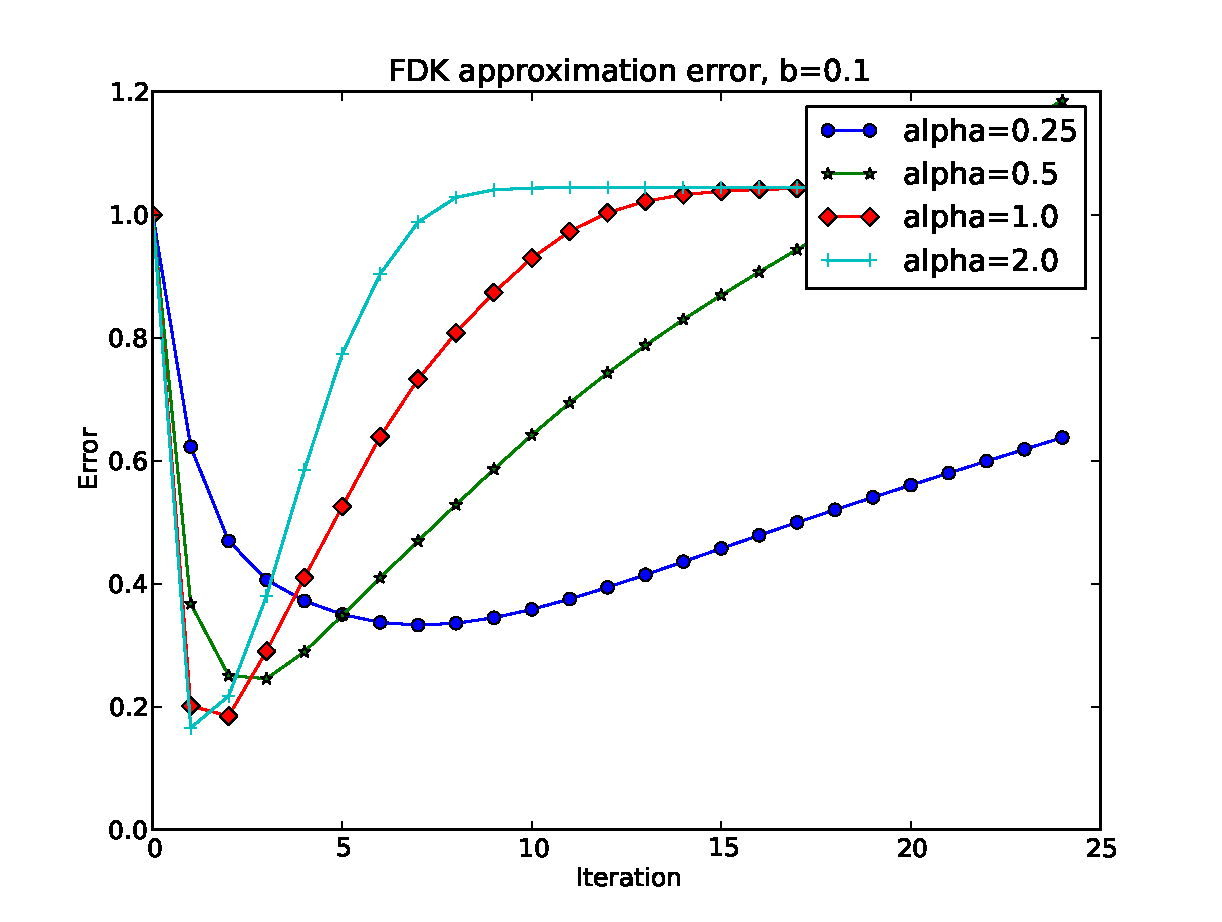
\includegraphics[width=\linewidth]{./figs/bumpyerr1.pdf}
  \endminipage
%\caption[Fitting an order 5 Fourier function with $b = .15$]
%{FDK fit for some order 5 Fourier function.}
\end{figure}

%\begin{figure}[!htb]
%  \minipage{0.12\textwidth}
%    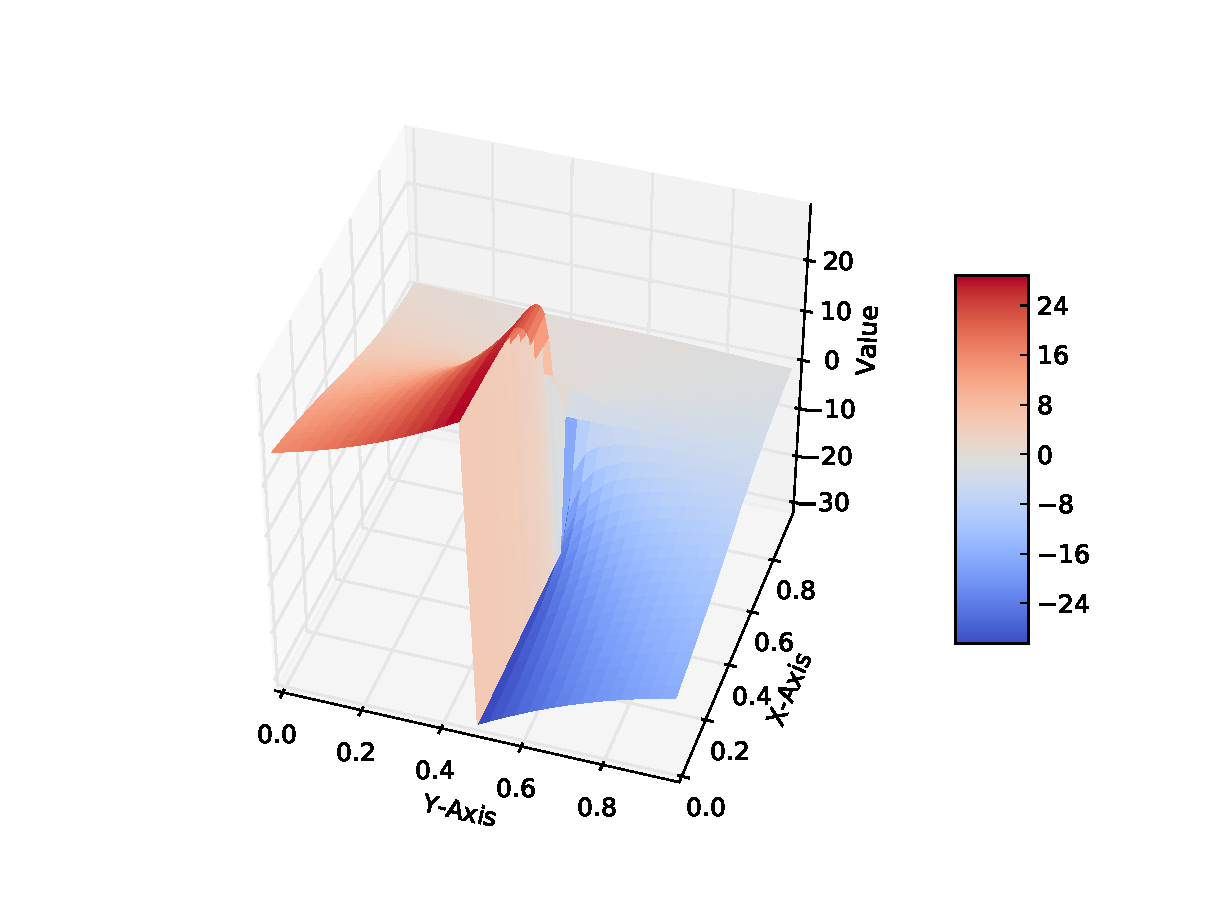
\includegraphics[width=\linewidth]{../writeup/figs/chap4/atan.pdf}
%  \endminipage\hfill
%  \minipage{0.12\textwidth}
%    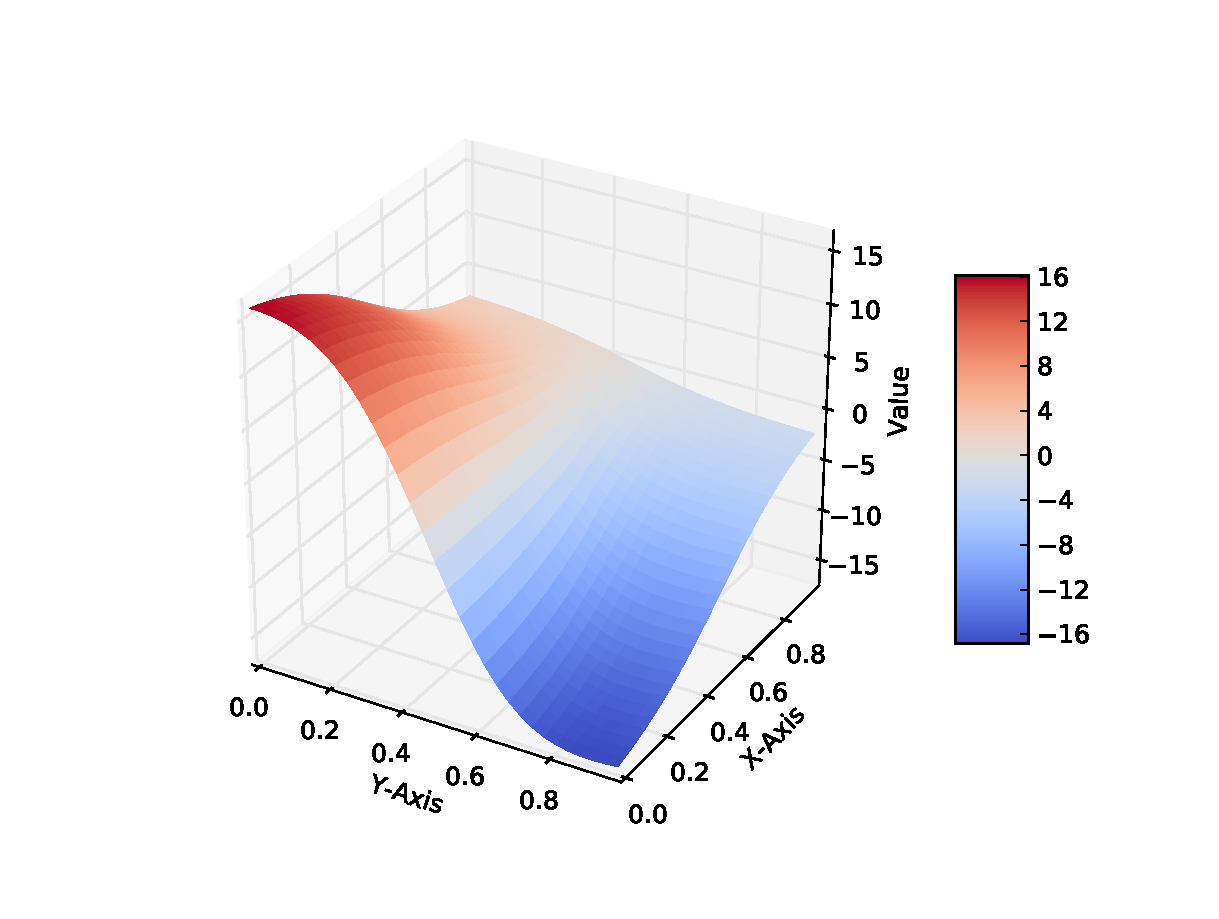
\includegraphics[width=\linewidth]{../writeup/figs/chap4/atan3s.pdf}
%  \endminipage
%  \minipage{0.12\textwidth}
%    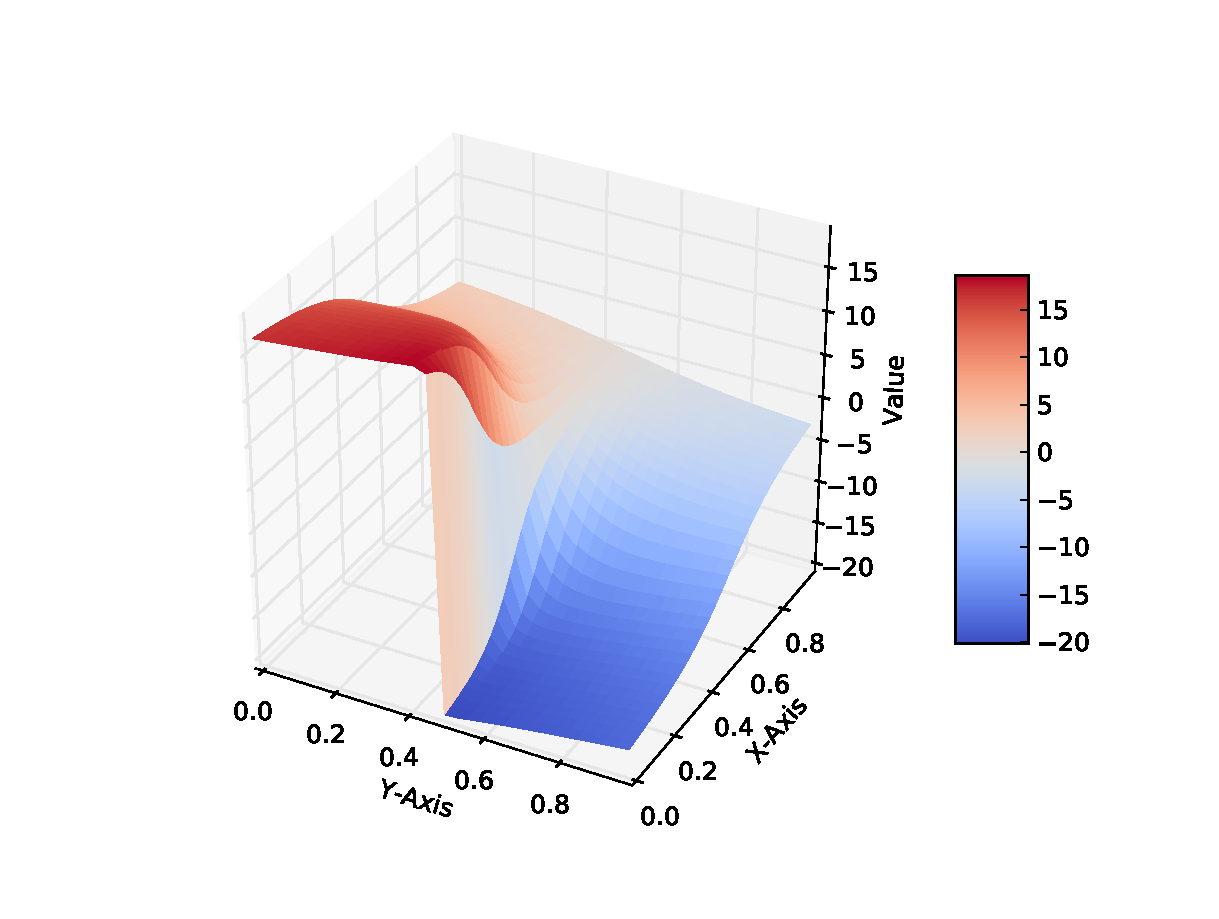
\includegraphics[width=\linewidth]{../writeup/figs/chap4/atan3e.pdf}
%  \endminipage
%  \minipage{0.12\textwidth}
%    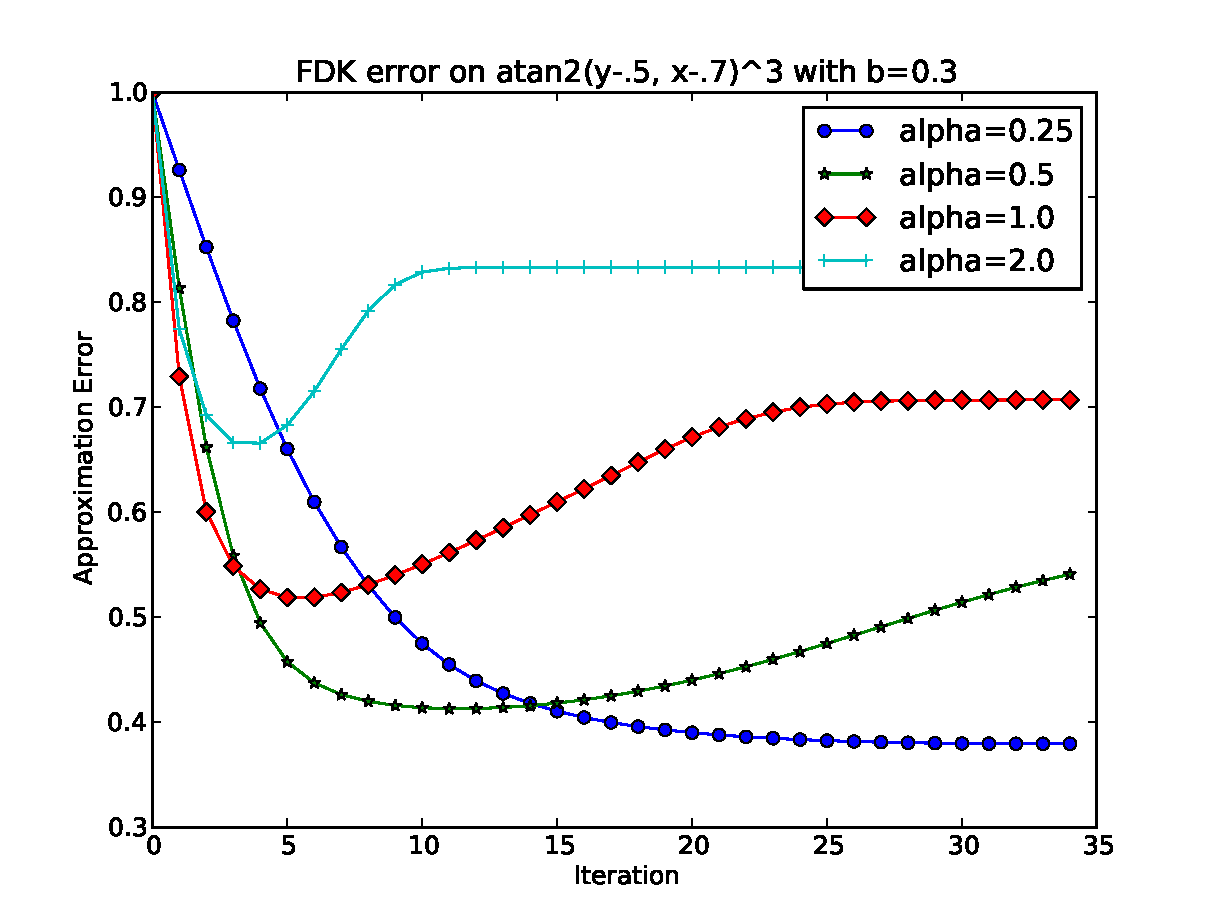
\includegraphics[width=\linewidth]{../writeup/figs/chap4/atanerr.pdf}
%  \endminipage
%\caption[Fitting the arctan]{Fitting $f(x,y) = \tan^{-1}(x - .7, y - .5)^3$.
%Left to right, the function being approximated, the kernel smoother fit, the best FDK fit,
%and the approximation errors over time.}
%\end{figure}

%\chapter{PinBall Trajectories}
This section shows the trajectories generated by KBSF (left) and DKBSF (right).
Each picture corresponds to a row in Table 5.1.
The trajectories generated by KBRL and DKBRL are not shown because they
were so similar to the ones in Figure 5-14.

\begin{figure}[!!!ht]
  \centering
    \includegraphics[width=110mm]{figs/apdx/f0.png}
\end{figure}

\begin{figure}[!!!ht]
  \centering
    \includegraphics[width=110mm]{figs/apdx/f1.png}
\end{figure}

\begin{figure}[!!!ht]
  \centering
    \includegraphics[width=110mm]{figs/apdx/f2.png}
\end{figure}

\begin{figure}[!!!ht]
  \centering
    \includegraphics[width=110mm]{figs/apdx/f3.png}
\end{figure}

\begin{figure}[!!!ht]
  \centering
    \includegraphics[width=110mm]{figs/apdx/f4.png}
\end{figure}

\begin{figure}[!!!ht]
  \centering
    \includegraphics[width=110mm]{figs/apdx/f5.png}
\end{figure}

\begin{figure}[!!!ht]
  \centering
    \includegraphics[width=110mm]{figs/apdx/f6.png}
\end{figure}

\begin{figure}[!!!ht]
  \centering
    \includegraphics[width=110mm]{figs/apdx/f7.png}
\end{figure}

\begin{figure}[!!!ht]
  \centering
    \includegraphics[width=110mm]{figs/apdx/f8.png}
\end{figure}

\begin{figure}[!!!ht]
  \centering
    \includegraphics[width=110mm]{figs/apdx/f9.png}
\end{figure}

\begin{figure}[!!!ht]
  \centering
    \includegraphics[width=110mm]{figs/apdx/f10.png}
\end{figure}


\end{document}
